\chapter{Higgs $\to \Pgt\Pgt$ via Associated Production}
\label{sec:vh_analysis}

This chapter describes a study of Higgs boson produced via the $\PW\PH$ and
$\PZ\PH$ associated production processes. The Higgs boson subsequently
decays to a pair of $\tau$ leptons and uses CMS proton-proton collision data gathered in 2016. 
This study provides the completion of the previously described
$\htt$ analysis in Section~\ref{sec:htt_analysis} and is performed 
using center-of-mass energy 13 TeV data from the LHC. Combining
the results from this associated production targeted analysis with the results 
of the gluon fusion and VBF targeted analysis
we produce the first single experiment observation of the $\htt$ process at 13 TeV, 
observed at the 5.5 $\sigma$ confidence level. 

This analysis uses the previously described proton-proton CMS dataset gathered during 2016 
corresponding to a total integrated luminosity of 35.9\fbinv.
For the $\PZ\PH$ search, $\PZ\rightarrow \Pe\Pe$
and $\PZ \to \Pgm\Pgm$ decays are considered combined with four possible $\Pgt\Pgt$ 
final states from the Higgs boson decay: $\Pe\tauh$, $\Pgm\tauh$,
$\Pe\Pgm$ and $\tauh\tauh$. For the $\PW\PH$ search, four final states are considered with
the $\PW$ boson decaying leptonically to an electron or muon, and at least one $\tauh$ from the Higgs leptons:
$\Pgm\Pgm\tauh$, $\Pe\Pgm\tauh$, $\Pe\tauh\tauh$ and $\Pgm\tauh\tauh$. 

There are many similarities between the gluon fusion and VBF targeted $\htt$ analysis
and the associated production targeted $\htt$ analysis. When appropriate, instead of repeating
what has already been documented in other chapters, I refer back to the appropriate sections.



\section{Overview}
This chapter specifically focuses on studying the Higgs boson produced via the associated
production mechanisms, $\PW\PH$/$\PZ\PH$. A study of the Higgs boson produced in the gluon fusion or VBF processes
is presented in Chapter~\ref{sec:htt_analysis}. This study utilizes the
full 2016 $\pp$ dataset collected by CMS corresponding to 35.9$\fbinv$ of integrated luminosity.
In the following pages the symbol $\ell$ refers to electrons and muons and $\tauh$ refers to hadronically
decaying $\tau$ leptons. We study all possible $\tau\tau$ final state combinations with the
exception of two electron and two muon final states because of the low 
$\tau\tau \to \tau_{e}\tau_{e}/\tau_{\mu}\tau_{\mu}$
branching fractions. The $\htt$ final states which are
studied are: $\tau_{e}\tauh$ denoted here as $\Pe\tauh$, $\tau_{\mu}\tauh$ denoted as $\Pgm\tauh$,
$\tau_{e}\tau_{\mu}$ denoted here as $\Pe\Pgm$, and lastly, $\tauh\tauh$ denoted as $\tauh\tauh$.
This combination of final states covers about 94\% of all possible $\tau\tau$ final states.
We ensure uniqueness between the studied channels be applying veto criteria to events based
on the number of reconstructed loosely identified electrons and muons. This ensures that 
no data or simulated event is double counted between the two $\htt$ studies or in 
multiple final states.



\subsection{Triggers}
Events in the $\PW\PH$ and $\PZ\PH$ production channels are selected using single or 
double lepton triggers, since the $\PW$ and $\PZ$ bosons ensure the presence of one 
or two well-isolated leptons with sufficiently high $\pt$. 
The $\PW\PH$ targeted final states rely on a set of single lepton triggers
which must be fired by the $\PW$ boson associated lepton. These single
lepton triggers are the same single electron and single muon triggers which are 
described in the $ggH$ and VBF targeted analysis described in 
Section~\ref{sec:htt_triggers}. In general, the $\PW$ boson associated lepton
will have a higher $\pt$ than the Higgs boson associated leptons providing
higher efficiency for trigger selection. By requiring that only the $\PW$
boson associated lepton fires the trigger, we ensure that there is negligible
bias in the selection of the Higgs boson associated leptons from the trigger
requirements. The non-biased Higgs boson associated lepton selection 
allows us to use specific background estimation techniques which are described
in the background estimation Section~\ref{sec:vh_background_estimation}.

The $\PZ\PH$ targeted final states utilize the presenece of the $\PZ$ boson
for passing trigger selections. Double electron and double muon triggers are used in these
final states. The presence of two simultaneous leptons in the double lepton
triggers allows for lower $\pt$ thresholds on each lepton which increases
the acceptance of $\PZ\PH$ events. The $\PZ$ boson associated electrons
or muons must be match to the leptons which fired the high level trigger.
Similar to the $\PW\PH$ final states, this removes selection bias from the
Higgs boson associate leptons and enables the use of specific background
estimation methods.

The trigger selection criteria for the $\PW\PH$ and $\PZ\PH$ targeted final 
states is detailed in Table~\ref{tab:vh_triggers}.


\begin{table*}[htbp]
\centering
\begin{small}
\begin{tabular}{lll}
     \multicolumn{3}{c}{$\PW\PH$ trigger selection requirements}                 \\ 
\hline
  Channel           &         Trigger ($\pt/\eta$)         & Lepton Selection: $\pt$     \\
\hline
 $\Pe\Pgm\tauh$      &  $\Pgm (22/2.1)$ or $\Pe (25/2.1)$  &     $\pt^\Pe>15, \pt^\Pgm>23$ or $\pt^\Pe>26, \pt^\Pgm>15$  \\ 
 $\Pgm\Pgm\tauh$     &  $\Pgm (22/2.1)$                    &     $\pt^\Pgm>23,\pt^\Pgm>15$                               \\ 
 $\Pe\tauh\tauh$     &  $\Pe (25/2.1)$                     &     $\pt^\Pe>26$                                            \\ 
 $\Pgm\tauh\tauh$    &  $\Pgm (22/2.1)$                    &     $\pt^\Pgm>23$                                           \\ 
\hline \\

\\
     \multicolumn{3}{c}{$\PZ\PH$ trigger selection requirements}                 \\ 
\hline
  Channel           &         Trigger ($\pt/\eta$)         & Lepton Selection: $\pt$             \\
\hline
  $\Pe\Pe\Pgm\tauh$     &                                    &                                   \\ 
  $\Pe\Pe\Pe\tauh$      & $\Pe(23/2.5)\,\&\,\Pe(12/2.5)$,    &  $\pt^\Pe>24\,\&\,\pt^\Pe>13$,    \\ 
  $\Pe\Pe\tauh\tauh$    & or $\Pe(27/2.5)$                   &  or $\pt^\Pe>28$                  \\ 
  $\Pe\Pe\Pe\Pgm$       &                                    &                                   \\ 
\hline
  $\Pgm\Pgm\Pgm\tauh$   &                                    &                                   \\ 
  $\Pgm\Pgm\Pe\tauh$    &  $\Pgm(17/2.4)\,\&\,\Pgm(8/2.4)$,  &  $\pt^\Pgm>18\,\&\,\pt^\Pgm>10$,  \\ 
  $\Pgm\Pgm\tauh\tauh$  &   or $\Pgm(24/2.4)$                &  or $\pt^\Pgm>25$                 \\ 
  $\Pgm\Pgm\Pe\Pgm$     &                                    &                                   \\ 
\hline
\end{tabular}
\end{small}
\caption{Kinematic selection requirements for $\PW\PH$ and $\PZ\PH$ events.
The trigger requirement is defined by a combination of trigger candidates with 
\pt over a given threshold (in \GeV), indicated inside parentheses. The 
pseudorapidity thresholds come from trigger and object reconstruction constraints.
The trigger requirements for the $\PZ\PH$ events are defined by the $\PZ$ boson
decay products, either $\PZ\to\Pe\Pe$ or $\PZ\to\Pgm\Pgm$.
\label{tab:vh_triggers}
}
\end{table*}



\subsection{Event Selection}
\label{sec:vh_evt_selection}
In the $\Pe\Pgm\tauh$ and $\Pgm\Pgm\tauh$ final states of the $\PW\PH$ channel, 
the two light leptons are required to have the same charge to reduce the $\ttbar$ 
and $\PZ+\textrm{jets}$ backgrounds where one or more jets is misidentified as a $\tauh$ 
candidate. The $\tauh$ candidate has opposite charge to the light leptons. The highest $\pt$
light lepton is considered as coming from the $\PW$ boson, while the Higgs boson 
candidate is formed from the $\tauh$ object and the subleading light lepton. The 
correct pairing is achieved in about 75\% of events. The leading light lepton is required 
to fire the single lepton triggers and to have a $\pt$ that is 1\GeV above the online 
thresholds, whereas the subleading light lepton has $\pt>15\GeV$ resulting from
optimization. Selection criteria based on three variables have been found to 
improve the results in both channels:
\begin{itemize}
\item $L_T>100\GeV$, where $L_T$ is the scalar $\pt$ sum of the three objects in the final state;
\item $\abs{\Delta\phi(\ell_1,\PH)}>2.0$, where $\ell_1$ is the leading light lepton, and 
$\PH$ is the system formed by the subleading light lepton and the $\tauh$ candidate;
\item $\abs{\Delta\eta(\ell_1,\PH)}<2.0$.
\end{itemize}


In the $\Pe\tauh\tauh$ and $\Pgm\tauh\tauh$ final states of the $\PW\PH$ channel, 
the $\tauh$ candidates are required to have opposite charge. As the result 
of an optimization, the $\tauh$ that has the same charge as the light lepton and must 
have $\pt > 35\GeV$, and for the subleading one, $\pt > 20\GeV$. This is driven 
by the fact that the $\tauh$ that has the same charge as the light lepton is almost 
always a jet misidentified as a $\tauh$ candidate, and the jet misidentification 
rate strongly decreases with $\pt$. Selection criteria based on three variables 
have been found to improve the results in both channels:
\begin{itemize}
\item $L_T>130\GeV$, where $L_T$ is the scalar $\pt$ sum of the three objects in the final state;
\item $\abs{\vec{S_T}}<70\GeV$, where $\vec{S_T}$ is the vectorial $\pt$ sum of the three objects in the final state and of $\etvecmiss$;
\item $\abs{\Delta\eta(\tauh,\tauh)}<2.0$.
\end{itemize}



In the $\PZ\PH$ final states, the $\PZ$ boson is reconstructed from the opposite charge, same-flavor
light lepton combination which has a mass closest to the $\PZ$ boson mass. Different 
electron and muon identification and isolation criteria are used for the leptons 
assigned to the $\PZ$ boson compare to those assigned to the Higgs boson. A looser
selection is applied for the $\PZ$ boson associated leptons to increase signal acceptance
while a tighter selection is applied to those assigned to the Higgs boson to
decrease the background contributions from $\PZ+\textrm{jets}$ and other reducible
backgrounds. The specific selections detailed in Table~\ref{tab:vh_inclusive_selection},
including those chosen for the $\tauh$ candidates, where chosen based on 
optimizing for best signal sensitivity.

To further suppress the contributions from the $\PZ+\textrm{jets}$ background, the signal 
region is split into a High-$L_{T}^{\textrm{Higgs}}$ and Low-$L_{T}^{\textrm{Higgs}}$
region where $L_{T}^{\textrm{Higgs}}$ is defined as the scalar $\pt$ sum of the decay 
products of the $\PH$ boson. Because of the identical event kinematics, the 
$L_{T}^{\textrm{Higgs}}$ regions are defined based on the $\htt$ final 
states of an event. The split between the High- and Low-$L_{T}^{\textrm{Higgs}}$
regions are:
\begin{itemize}
\item $\ell\ell\Pe\tauh$: $L_{T}^{\textrm{Higgs}} = 60\GeV$
\item $\ell\ell\Pgm\tauh$: $L_{T}^{\textrm{Higgs}} = 60\GeV$
\item $\ell\ell\tauh\tauh$: $L_{T}^{\textrm{Higgs}} = 75\GeV$
\item $\ell\ell\Pe\Pgm$: $L_{T}^{\textrm{Higgs}} = 50\GeV$
\end{itemize}
For convenience, the High- and Low-$L_{T}^{\textrm{Higgs}}$ regions are plotted
side-by-side.



\subsection{Baseline Object Selection}
\label{sec:vh_obj_selection}

The expression $\pt^{\ell}$ stands for the $\pt$ of the lepton. The isolation 
requirements used in this analysis, based on $I^{\ell}$~\ref{eqn:rel_isolation}, 
are listed in Table~\ref{tab:vh_inclusive_selection}.
In the associated production analysis we reject events which have been tagged as likely
including heavy flavor jet decays from b-quarks.
The working point chosen 
in this analysis gives an efficiency for real b jets of about 70\% for 
about 1\% of light flavor or quark jets being misidentified~\ref{sec:reco_b_jet}.
For negligible signal loss, this requirements significantly decreases the $\ttbar$,
$\ttbar+\PW$, and $\ttbar+\PZ$ background contributions.

The $\tauh$ candidates are identified using the MVA discriminant discussed in
Section~\ref{sec:obj_reco_tau}.
Three $\tauh$ MVA working points are used in this analysis,
\texttt{Very Tight}, \texttt{Tight}, and \texttt{Medium Tau MVA} ID. Each working point was selected based on
optimizing the analysis for highest sensitivity to the associated production
$\htt$ processes. 

A summary of the object selection details for each final state in the associated
production analysis is in Table~\ref{tab:vh_inclusive_selection}.
All reconstructed objects in the events are required to be separated from each 
other by $\Delta R > 0.3$. In the case of $\tauh$, they are required to be 
separated from all other objects by $\Delta R > 0.5$. The resulting event samples are made mutually 
exclusive by discarding events that have additional loosely identified 
and isolated muons or electrons.

\begin{table*}[htbp]
\centering
\begin{small}
\begin{tabular}{ll}
     \multicolumn{2}{c}{$\PW\PH$ selection requirements}                 \\ 
     \multicolumn{2}{c}{$\pt^{\tauh}>20$, $|\eta^{\tauh}|<2.3$, $I^\Pe<0.1$, $I^\Pgm<0.15$, b-veto }                 \\ 
\hline
  Channel           &       Lepton Selection: Iso.  \\
\hline
 $\Pe\Pgm\tauh$      &  \texttt{Tight Tau MVA}  \\
 $\Pgm\Pgm\tauh$     &  \texttt{Tight Tau MVA}  \\
 $\Pe\tauh\tauh$     &  \texttt{Medium/Very Tight Tau MVA} \\
 $\Pgm\tauh\tauh$    &  \texttt{Medium/Very Tight Tau MVA} \\
\hline \\

\\
     \multicolumn{2}{c}{$\PZ\PH$ selection requirements}                 \\ 
     \multicolumn{2}{c}{$\PZ$ boson reconstructed from opposite charge, same-flavor light leptons, $60\GeV < \textrm{m}_{\ell\ell} < 120\GeV$}  \\ 
     \multicolumn{2}{c}{$\tauh$ baseline requirements: $\pt^{\tauh}>20$, $|\eta|<2.3$, MVA $\tauh$ Medium}   \\ 
     \multicolumn{2}{c}{$\Pe$ baseline requirements: $\pt^\Pe>10$, $|\eta|<2.5$, MVA Loose ID }   \\ 
     \multicolumn{2}{c}{$\Pgm$ baseline requirements: $\pt^\Pgm>10$, $|\eta|<2.4$, ID Loose, $I^\Pgm<0.25$ }   \\ 
\hline
  Channel           &          Lepton Selection: Isolation  \\
\hline
  $\Pe\Pe\Pgm\tauh$     &   $I^\Pgm<0.15$       \\
  $\Pe\Pe\Pe\tauh$      &   $\Pe$ Tight ID, $I^\Pe<0.15$ \\
  $\Pe\Pe\tauh\tauh$    &   baseline selection       \\
  $\Pe\Pe\Pe\Pgm$       &   $\Pe$ Tight ID, $I^\Pe<0.15$, $I^\Pgm<0.15$ \\
\hline
  $\Pgm\Pgm\Pgm\tauh$   &   $I^\Pgm<0.15$       \\
  $\Pgm\Pgm\Pe\tauh$    &   $\Pe$ Tight ID, $I^\Pe<0.15$ \\
  $\Pgm\Pgm\tauh\tauh$  &   baseline selection       \\
  $\Pgm\Pgm\Pe\Pgm$     &   $\Pe$ Tight ID, $I^\Pe<0.15$, $I^\Pgm<0.15$ \\
\hline
\end{tabular}
\end{small}
\caption{
Electron, muon and $\tauh$ selection criteria for each final state in the
associated production $\htt$ analysis.
}
\label{tab:vh_inclusive_selection}
\end{table*}



\section{Data Set}
\label{sec:vh_dataset}
The associated production targeted $\htt$ study utilizes the same dataset as the
$ggH$ and VBF targeted study. The dataset used is the full 2016 $\pp$ 
dataset collected by CMS corresponding to 35.9$\fbinv$ 
of integrated luminosity. The data were gathered at center-of-mass energy 13 TeV.
For further details see Section~\ref{sec:htt_dataset}.



\section{Monte Carlo Samples}
\label{sec:vh_mc_samples}
Signal and background processes are modeled with samples of simulated events.
For details on the production for simulated events, see section~\ref{sec:simulation}.
%Because the analysis focuses on
%measuring the $\PW\PH$ and $\PZ\PH$ processes, the $\ttbar\PH$ process is 
%included as background.

For each simulated event, a number of additional pileup interactions is simulated and added. 
The number of pileup interactions added is based on best efforts to match the simulated
events to the pileup in data which is estimated from the measured instantaneous
luminosity for each bunch crossing. The average number of additional pileup interactions in
the 2016 CMS data is approximately 27 interactions per bunch crossing.



\section{SVFit Algorithm}
The visible mass of the $\Pgt\Pgt$ system, $\mvis$, can be used to separate
the $\PH\to \Pgt \Pgt$ signal events
from the large contribution of irreducible $\PZ \to \Pgt \Pgt$ events.
However, the neutrinos from the $\Pgt$ lepton decays carry a large fraction of
the $\Pgt$ lepton energy and reduce the discriminating power of this variable.
The \textsc{svfit} algorithm used in the $ggH$ and VBF targeted analysis
and discussed in Section~\ref{sec:svfit} is used in the associated production
analysis as well. It combines the \etvecmiss 
with the four-vectors of both $\Pgt$ candidates to calculate a more accurate 
estimate of the mass of the parent boson and is denoted as $\mtt$. The resolution 
of $\mtt$ is between 15 and 20\% depending on the $\Pgt\Pgt$ final state. The 
$\mtt$ variable is used in the $\PZ\PH$ channel where the majority of 
\etvecmiss is attributable to the $\Pgt$ decays. The variable $\mvis$ is used in the 
$\PW\PH$ channel because the \textsc{svfit} algorithm cannot properly account for the 
additional \etvecmiss associated with the neutrino from the $\PW$ boson decay. 



\section{Background Estimation}
\label{sec:vh_background_estimation}

The irreducible backgrounds for the associated production analysis can
be split into those for the $\PZ\PH$ four lepton final and those
with three lepton final states. When a lepton escapes the fiducial
volume of the detector or is otherwise poorly reconstructed, the four
lepton irreducible backgrounds can populate the $\PW\PH$ three
lepton final states as well.
Backgrounds typically with four or more genuine leptons composing
the irreducible background for the $\PZ\PH$ final states are: $\PZ\PZ$, 
$\ttbar\PZ$, $\PW\PW\PZ$, $\PW\PZ\PZ$, and $\PZ\PZ\PZ$. The dominant
three lepton irreducible backgrounds for the $\PW\PH$ final states are:
$\PW\PZ$ and $\ttbar \PW$. The irreducible backgrounds are 
estimated from simulations and scaled to their theoretical cross section. Higgs 
boson decays to pairs of $\PW$ or $\PZ$ bosons 
are also estimated from simulations and considered as background processes. 
Additionally, the $\ttbar\PH$ production process with all Higgs boson decay
paths is estimated from simulations and considered a background processes.

The reducible backgrounds, which have at least one jet misidentified as an electron, 
muon, or $\tauh$ candidate, are estimated from data. 
Data events meeting specific requirements detailed below are reweighted 
as a function of a misidentification rate to estimate the 
contribution of processes with jets misidentified as leptons in the signal region. 

In the $\PW\PH$ final states, the misidentification rate of jets as electrons, muons, 
or $\tauh$ candidates is measured in $\PZ+\textrm{jets}$ events. The $\PZ$ boson is reconstructed 
in its dielectron decay mode for measuring the jet to muon  misidentification
rate, and is reconstructed in its dimuon decay mode for measuring the jet to electron
or $\tauh$ misidentification rate.
The rates are measured in bins of the lepton $\pt$, and are 
split between reconstructed decay mode for the $\tauh$ candidates. 

In the $\Pe\Pgm\tauh$ and $\Pgm\Pgm\tauh$ final states, 
events are selected for reweighting if they pass the full signal region 
selection except that the subleading light lepton or the $\tauh$ do not 
pass the isolation or identification conditions.
To remove double-counting of events, events in simulation that have a jet that is 
misidentified as the $\tauh$ or as the subleading lepton, are discarded. Simulated 
events that have a jet misidentified as the leading $\PW$ boson associated lepton, but two real leptons 
for the Higgs boson associated subleading lepton and $\tauh$, are estimated from simulations as their 
contribution is not taken into account with the misidentification rate method 
described above. Such events mostly arise from $\ttbar$ and $\PZ+\textrm{jets}$ processes, 
and account for a small fraction of the total expected background in the signal region. 
In the $\Pe\tauh\tauh$ and $\Pgm\tauh\tauh$ final states of the $\PW\PH$ channels, 
the method is essentially the same, except that the object susceptible to being misidentified,
thus having the misidentificantion estimation method applied to it, 
is the $\tauh$ candidate that has the same charge as the light lepton.  

In the $\PZ\PH$ final states, a very similar misidentification rate is used
to estimate the contribution of jets misidentified as electrons, muons, or $\tauh$
candidates to the signal region events. The misidentification rate is measured in four object final states which
is dominated by $\PZ+\textrm{jets}$ events with a small contribution from 
$\ttbar$ events. Identical to the $\PW\PH$ final states, the rates are measured 
in bins of the lepton $\pt$, and are split between reconstructed decay modes for 
the $\tauh$ candidates. 

In these four lepton final states, the objects most susceptible 
to being misidentified jets are the $\PH$ boson associated objects.
In the $\PZ\PH$ final states, data events which pass the full
signal region selection, except either or both of the $\PH$ boson associated objects
fail identification or isolation criteria, are weighted by the misidentification
rate for the failing object and are assigned to the ``jet fakes'' background.
To avoid double counting, events with both $\PH$ boson associated objects failing have their weight
subtracted from the events which only have a single object failing. 
This misidentification rate method is used to estimate the yield of the reducible
backgrounds. The shape of the reducible background contribution is taken from
data in the signal free region with same charge objects assigned to the $\PH$ boson.
A high statistics, relaxed identification and isolation selection is used to reduce
statistical uncertainties. Kolmogorov-Smirnov tests have been performed to validate
shape compatibility between this relaxed same charge selection and the signal region
reducible background distributions.



\section{Monte Carlo Corrections}
\label{sec:vh_mc_corrections}



\section{Systematic uncertainties}
\label{sec:vh_systematics}
\subsection{Uncertainties related to object reconstruction and identification}
\subsection{Background estimation uncertainties}
\subsection{Signal prediction uncertainties}
\subsection{Other uncertainties}
\subsection{Luminsity}
\subsection{Lepton ID and Isolation}
\subsection{Tau Fake Rate}
\subsection{Energy Scales}
\subsubsection{Tau Energy Scale}
\subsubsection{Jet Energy Scale}
\subsubsection{MET Energy Scale}
\subsection{Theoretical Uncertainties for Higgs Boson}

Diff RB
MET - not applied to all WH

SAME
$\tauh$ identification efficiency for genuine $\tauh$
visible energy scale of genuine $\tauh$ leptons
uncertainties in the muon and electron identification, isolation, and trigger
rate uncertainty related to discarding events with a b-tagged jet
\etvecmiss scale uncertainties
    WH skipped
uncertainty in the integrated luminosity
finite number of simulated events



%The overall uncertainty in the $\tauh$ identification efficiency for genuine $\tauh$ 
%leptons is 5\%, which has been measured with a tag-and-probe method in $\PZ\to\Pgt\Pgt$ events.
%This number is not fully correlated among the various channels because the $\tauh$ 
%candidates are required to pass different working points of the discriminators that 
%reduce the misidentification rate of electrons and muons as $\tauh$ candidates.
%
%An uncertainty of 1.2\% in the visible energy scale of genuine $\tauh$ leptons 
%affects both the distributions and yields of the signals and backgrounds. It is 
%uncorrelated among the 1-prong, 1-prong + $\PGpz$, and 3-prong decay modes.
%
%The uncertainties in the muon and electron identification, isolation, and trigger 
%efficiencies lead to a rate uncertainty of 2\% for both muons and electrons.
%The uncertainty in the electron energy scale, which amounts to 2.5\% in the endcaps 
%and 1\% in the barrel of the detector, affects the final distributions and rate.
%In all channels, the effect of the uncertainty in
%the muon energy scale is negligible.
%
%The rate uncertainty related to discarding events with a b-tagged jet is
%4.5\% for processes with heavy-flavor jets, and 0.15\% for processes with light-flavor jets.



Uncertainties from the renormalization and the factorization scales, and from the 
choice of the PDF set, are taken into account for the $\PZ\PZ$ and $\PW\PZ$ 
background processes. The uncertainty from the renormalization and factorization 
scales is determined by varying these scales between 0.5 and 2 times their nominal 
value while keeping their ratio between 0.5 and 2. It leads to yield uncertainties 
of $^{+3.2\%}_{-4.2\%}$ for the $\Pq\Pq\rightarrow \PZ\PZ$ background, and $\pm 3.2\%$ 
for the $\PW\PZ$ process. The uncertainty from the PDF set is determined following 
the PDF4LHC recommendations, and leads to yield uncertainties of $+3.1/-4.2\%$ for 
the $\Pq\Pq\rightarrow \PZ\PZ$ background, and $\pm 4.5\%$ for the $\PW\PZ$ process. 
In addition, a 10\% uncertainty in the k-factor used for the $\Pg\Pg \rightarrow 
\PZ\PZ$  prediction is considered.  The uncertainty in the cross section of the 
rare $\ttbar\PW$ and $\ttbar\PZ$ processes amounts to 25\%.

The reducible backgrounds are estimated using the measured rates for jets to be 
misidentified as electrons, muons, or $\tauh$. The misidentification rates are 
measured in different bins of lepton $\pt$, and are further split between 
reconstructed decay modes for the $\tauh$. In the $\PW\PH$ final states where
the shape of the reducible background is take from the misidentification rate
method, the statistical uncertainty in every 
bin is considered as an independent uncertainty, which is propagated to the mass 
distributions and to the yields of the reducible background estimate. Rate
uncertainties applied in the $\PZ\PH$ final states cover this possible fluctuation
in rate from these uncertainties and, with the shape taken from the same charge
region, the shape is already validated a compatible.
In both the $\PW\PH$ and $\PZ\PH$ final states, an additional
uncertainty on the misidentification rates arising from the subtraction of 
prompt leptons estimated from simulations is taken into account and propagated to 
the reducible background mass distributions. 

In the $\PW\PH$ channels, an 
additional uncertainty comes from potentially different misidentification rates 
in $\PZ$ + jets events, where the rates are measured, and in $\PW$ + jets or 
$\ttbar$ events, which constitute a large fraction of the reducible background 
in the signal region. This leads to a 10\% yield uncertainty for the reducible 
background in each final state of the $\PW\PH$ final states. In the $\PZ\PH$ final
states a similar uncertainty is applied based on potential differences in the
measurement region versus the application region. These uncertainties
range from 26\% in the $\ell\ell\Pgm\tauh$ final states to 100\% in the
$\ell\ell\Pe\Pgm$ final states. The large uncertainty in the $\ell\ell\Pe\Pgm$ 
final states results from the very low expected reducible background yields 
which makes any comparison of the method susceptible to large statistical fluctuations.

%The \etvecmiss scale uncertainties~\cite{CMS-JME-12-002}, which are computed 
%event-by-event, affect the normalization of various processes through the event 
%selection, as well as their distributions through the propagation of these 
%uncertainties to the di-$\Pgt$ mass $\mtt$ in the $\PZ\PH$ channels. The 
%\etvecmiss scale uncertainties arising from unclustered energy deposits in the 
%detector come from four independent sources related to the tracker, ECAL, HCAL, 
%and forward calorimeters subdetectors. Additionally, \etvecmiss scale 
%uncertainties related to the uncertainties in the jet energy scale measurement, 
%which lead to uncertainties in the \etvecmiss calculation, are taken into 
%account. 

The rate and acceptance uncertainties for the signal processes related to the 
theoretical calculations are due to uncertainties in the PDFs, variations of 
the QCD renormalization and factorization scales, and uncertainties in the 
modeling of parton showers. The magnitude of the rate uncertainty depends on 
the production process and on the event category.

The inclusive uncertainty related to the PDFs amounts to 1.9 and 1.6\%, 
respectively, for the $\PW\PH$, and $\PZ\PH$ production modes~\cite{deFlorian:2016spz}. The
corresponding uncertainty for the variation of the renormalization and 
factorization scales is 0.7 and 3.8\%, respectively~\cite{deFlorian:2016spz}.

%The uncertainty in the integrated luminosity amounts to 2.5\%~\cite{CMS-PAS-LUM-17-001}.

%Uncertainties related to the finite number of simulated events, or to the 
%limited number of events in data control regions, are taken into account. They 
%are considered for all bins of the distributions used to extract the results.
%They are uncorrelated across different samples, and across bins of a single distribution. 

The systematic uncertainties considered in the analysis are summarized in Table~\ref{tab:vh_uncertainties}.

\begin{table*}[!ht]
\centering
\newcolumntype{x}{D{,}{\text{--}}{2.2}}
\begin{tabular}{ll}
Source of uncertainty & Magnitude \\
\hline
 $\tauh$ energy scale                & 1.2\% in energy scale\\
 $\Pe$ energy scale               & 1--2.5\%  in energy scale \\
 $\etvecmiss$ energy scale              & Dependent upon $\pt$ and $\eta$ \\
 $\tauh$ ID \& isolation & 5\% per $\tauh$  \\
 $\Pe$ ID \& isolation \& trigger  &   2\%  \\
 $\Pgm$ ID \& isolation \& trigger & 2\%  \\
 Diboson normalization & 5\% \\
 Integrated luminosity     & 2.5\%  \\
 b-tagged jet rejection & 4.5\% heavy flavor, 0.15\% light flavor \\
 Limited number of events                & Statistical uncertainty in individual bins  \\
 Signal theoretical uncertainty  & Up to 20\% \\
 Reducible background uncertainties & $\PW\PH$: shape and yield based \\
                                    & $\PW\PH$: 10\% yield \\
                                    & $\PZ\PH$: 26--100\% yield \\
\hline
\end{tabular}
\caption{Sources of systematic uncertainty.}
\label{tab:vh_uncertainties}
\end{table*}



\section{Results}
\label{sec:vh_results}


In the $\PZ\PH$ final states, the $\mtt$ distribution is
used for signal extraction. The Low-$L_{T}^{\textrm{Higgs}}$ and
High-$L_{T}^{\textrm{Higgs}}$ regions are plotted side-by-side
in the following distributions. 
%Figs.~\ref{fig:zh_results_svFitLLXX} 
Figs.~\ref{fig:zh_all_eight1}, ~\ref{fig:zh_all_eight2}, 
and \ref{fig:zh_results_svFitAll} show the
$\mtt$ distributions for each of the $\PZ\PH$ final states and
the combined distribution for all eight $\PZ\PH$ channels.
The eight $\PZ\PH$ final states are each fit separately in the global
fit; combining them together helps reduce statistical
fluctuations for visualization purposes only.
The distributions are post-fit and show full uncertainties.
The $\PW\PH$ and $\PZ\PH$ signals are shown as 5x larger than their best-fit
signal strength value of $2.5 \times$ SM.

\begin{figure}[h!]
 \begin{center}
  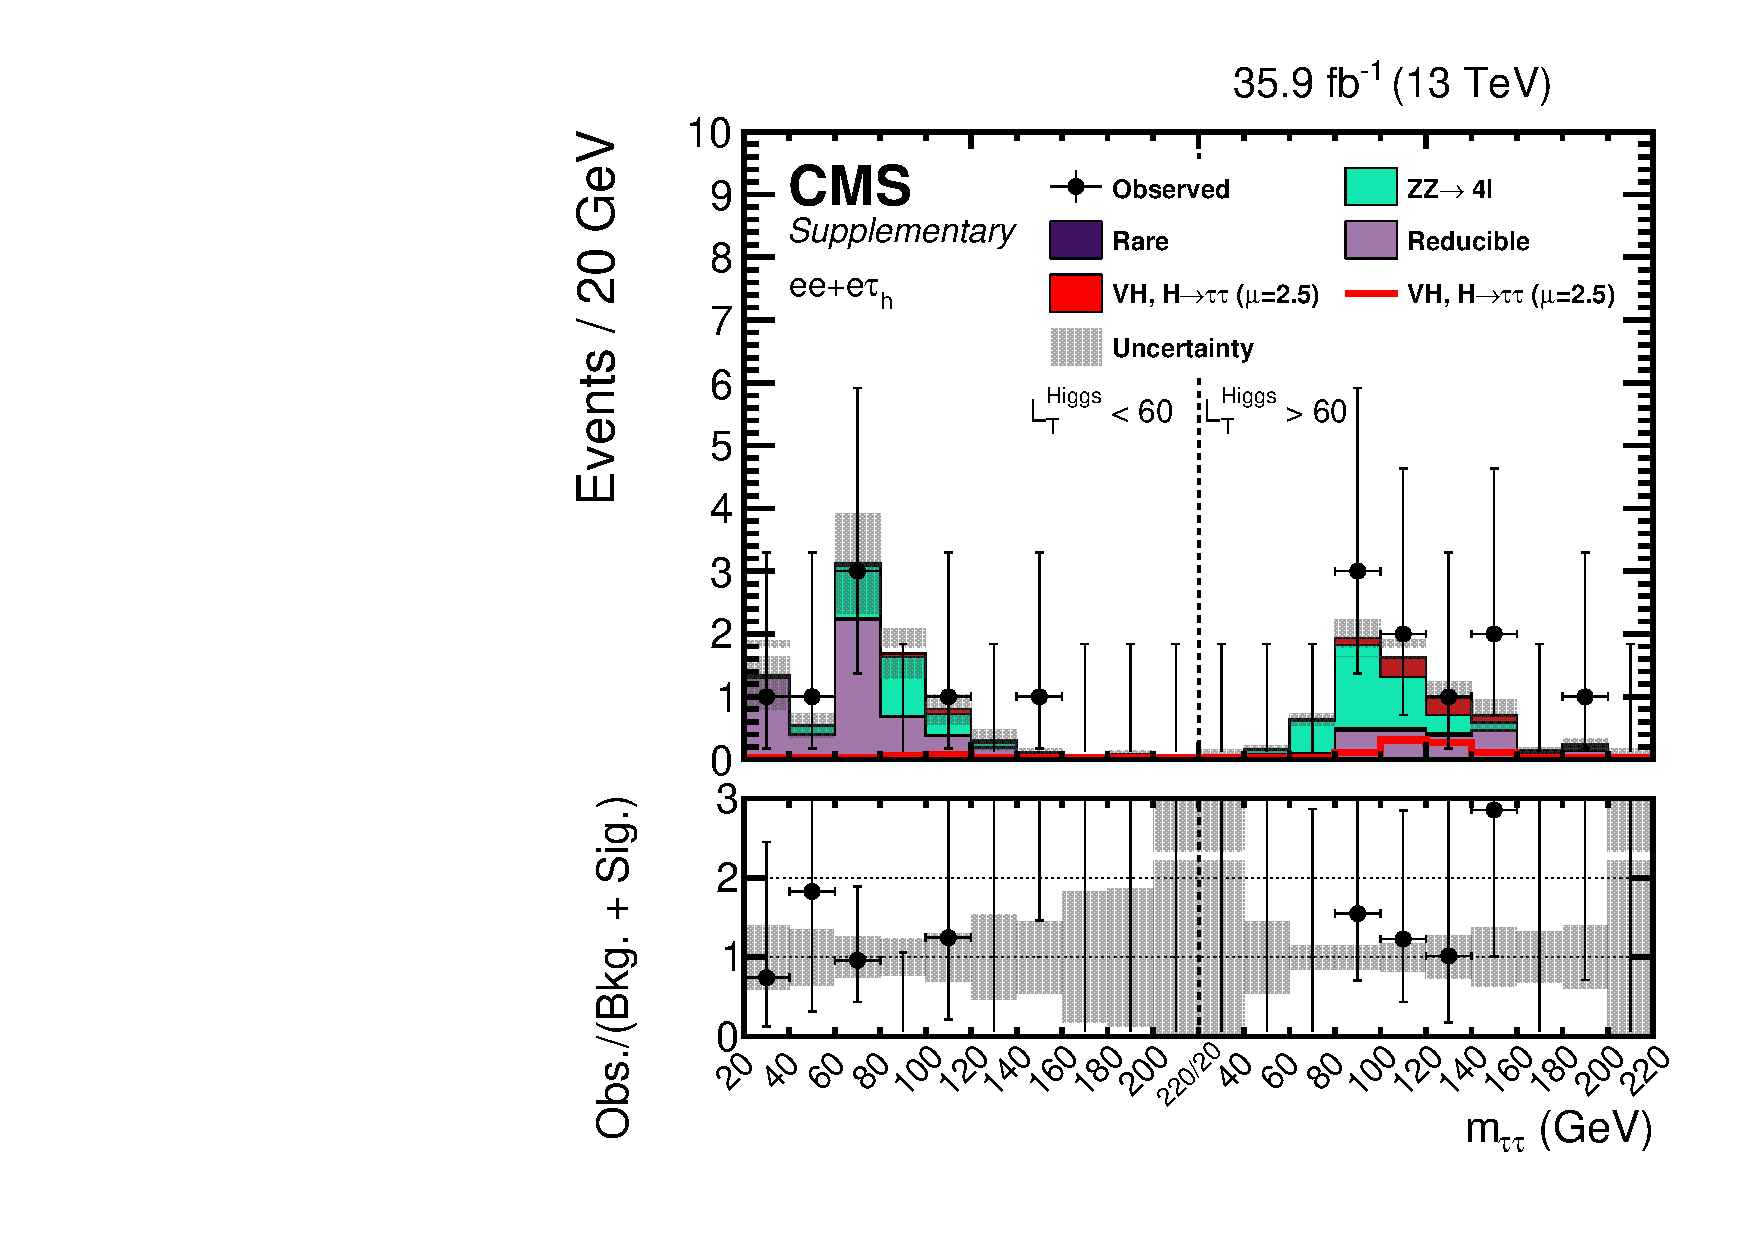
\includegraphics[width=0.45\textwidth]{higgs_to_taus_vh/plots/zh/eeet_postfit.pdf}
  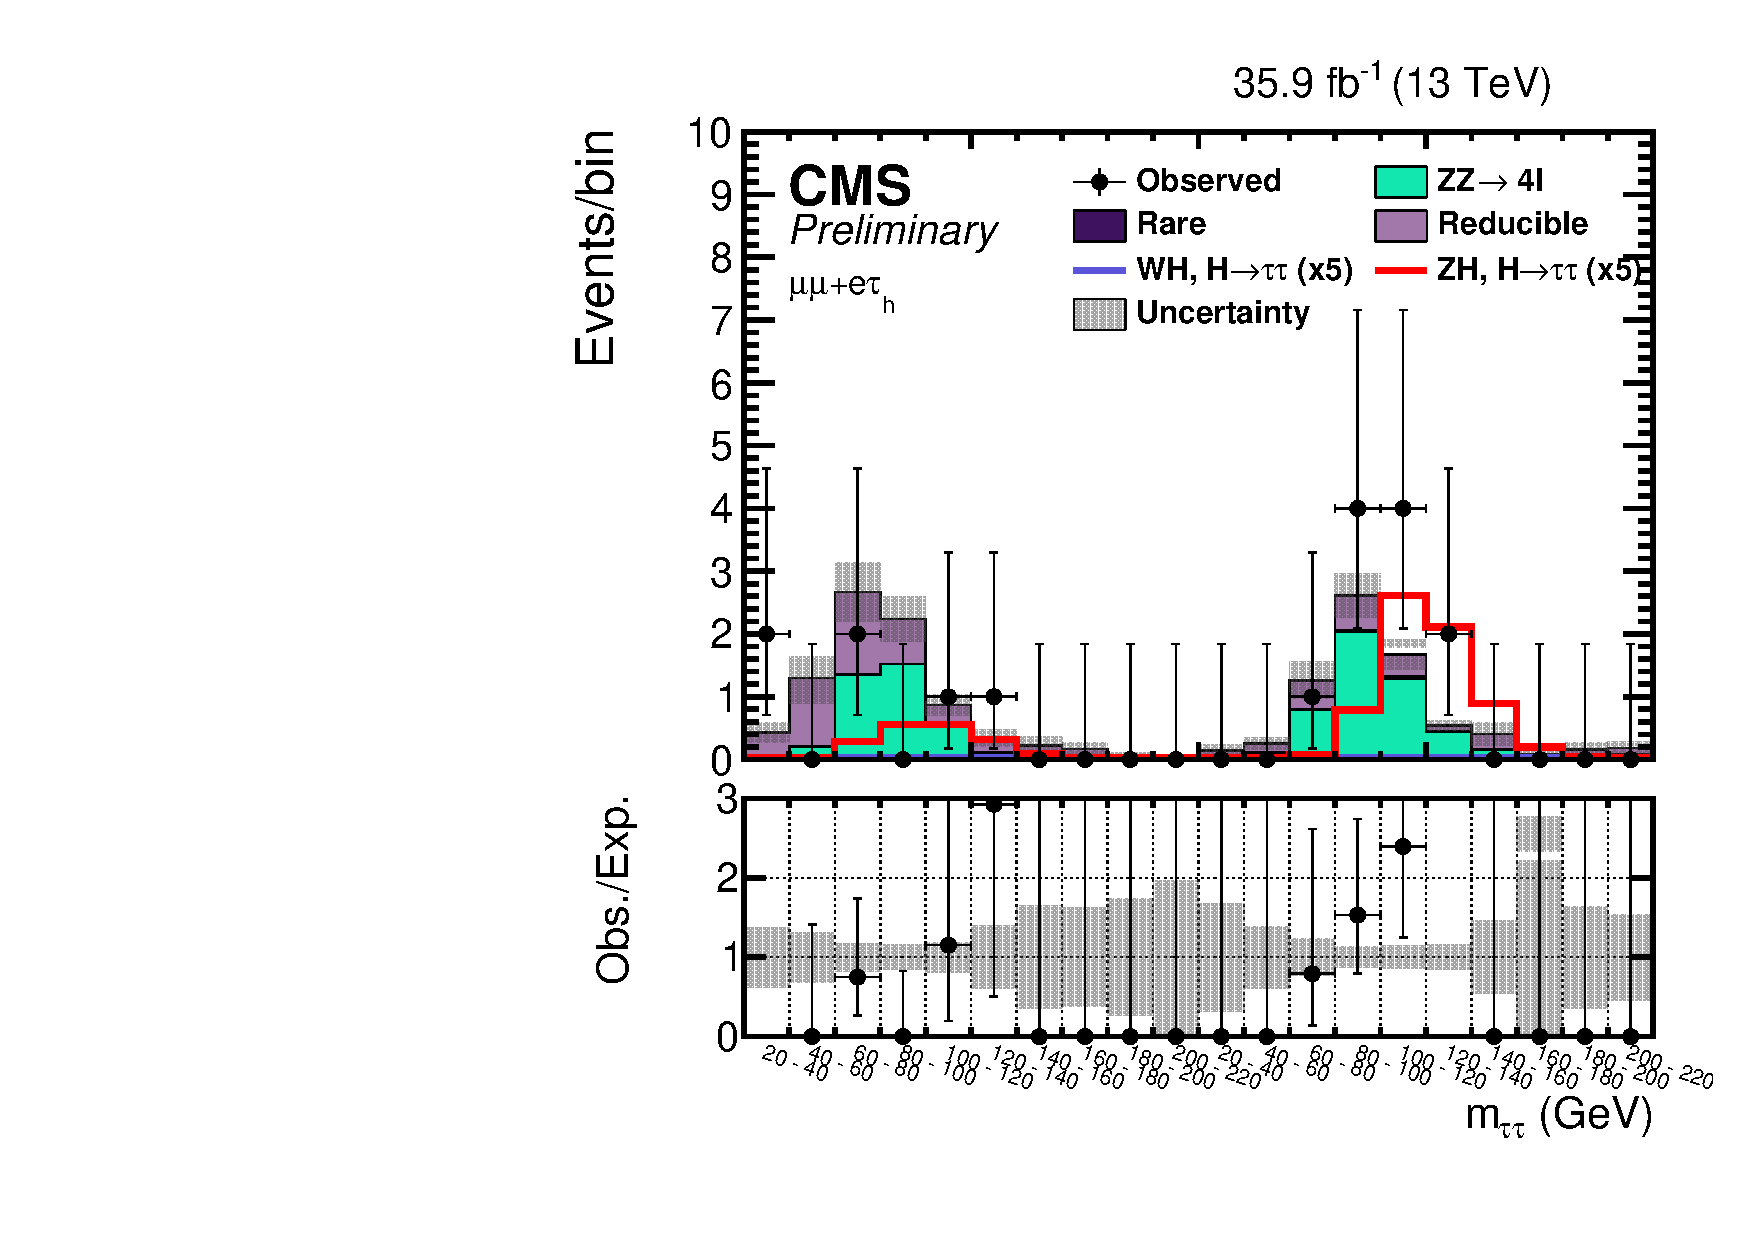
\includegraphics[width=0.45\textwidth]{higgs_to_taus_vh/plots/zh/emmt_postfit.pdf}
  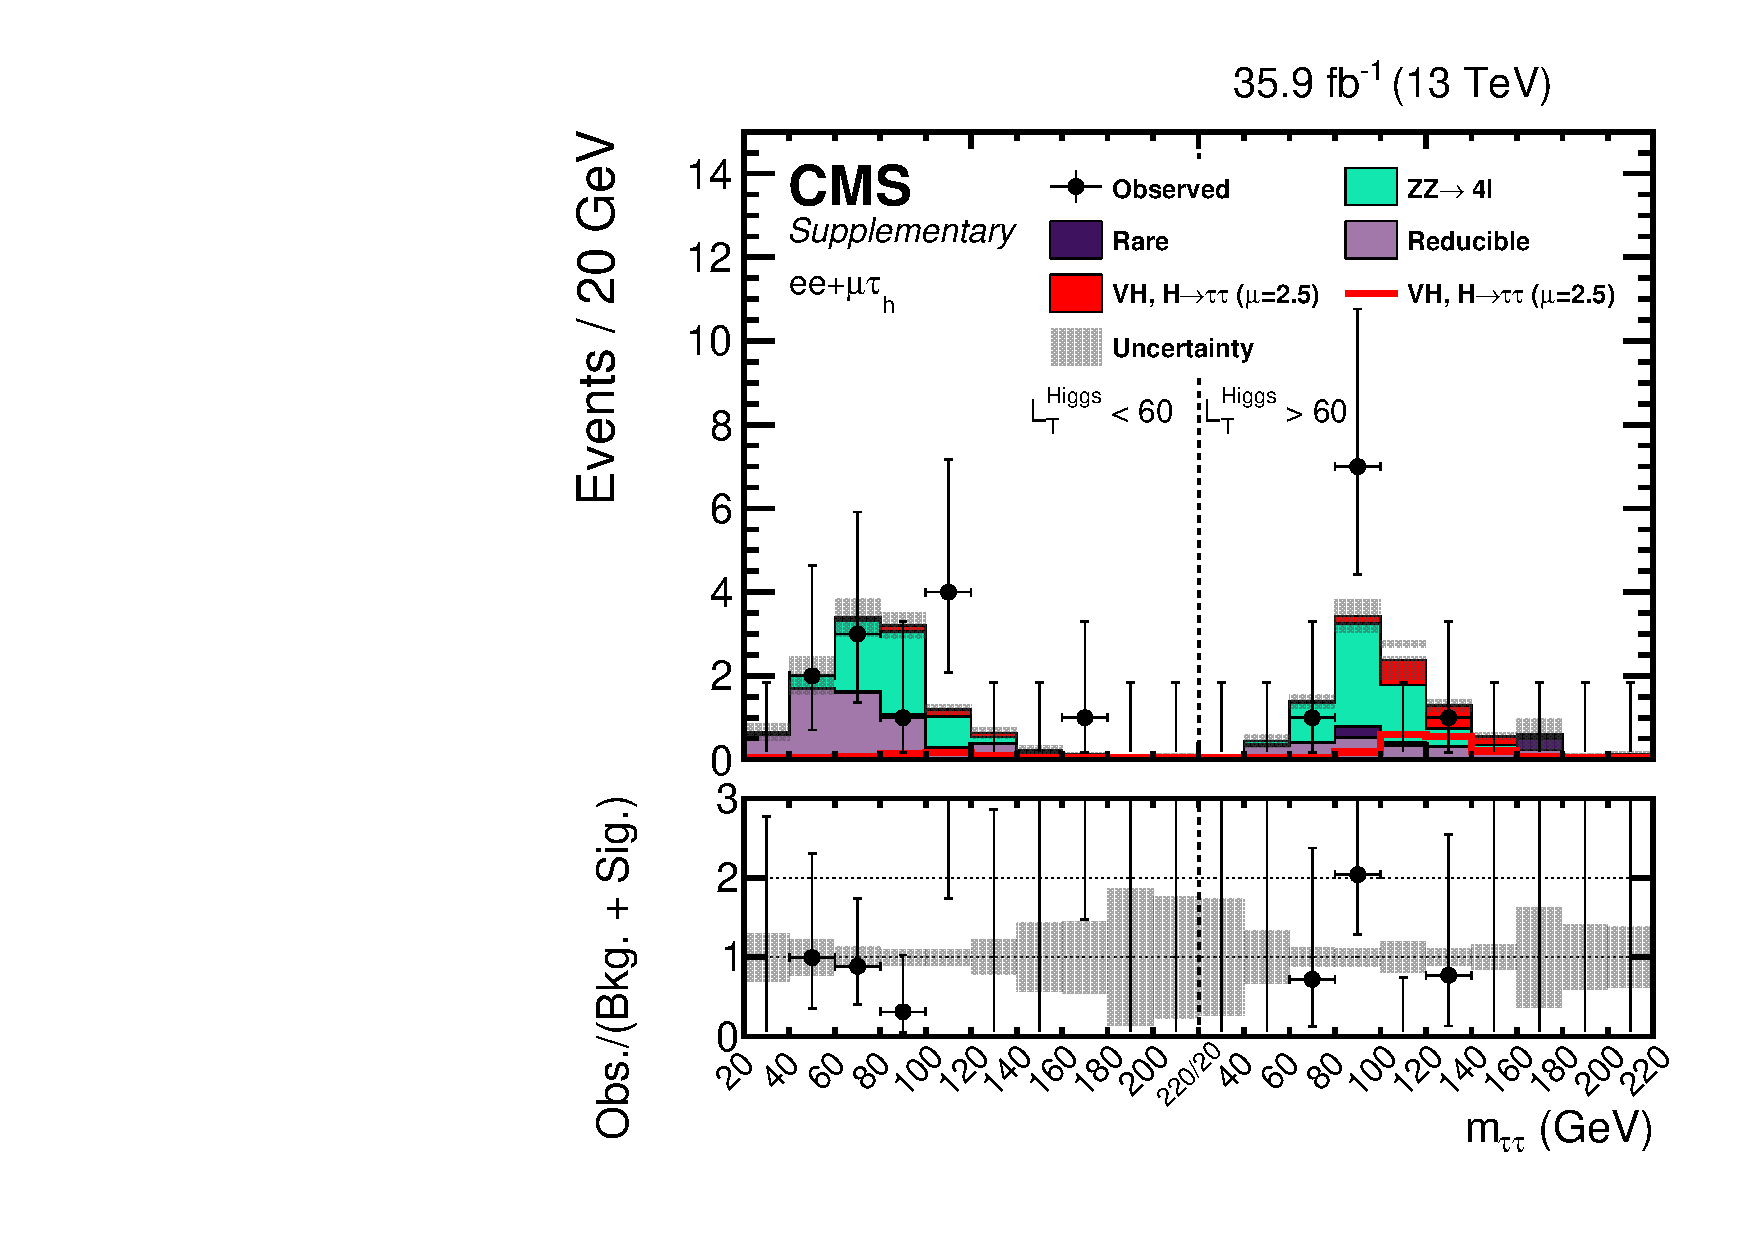
\includegraphics[width=0.45\textwidth]{higgs_to_taus_vh/plots/zh/eemt_postfit.pdf}
  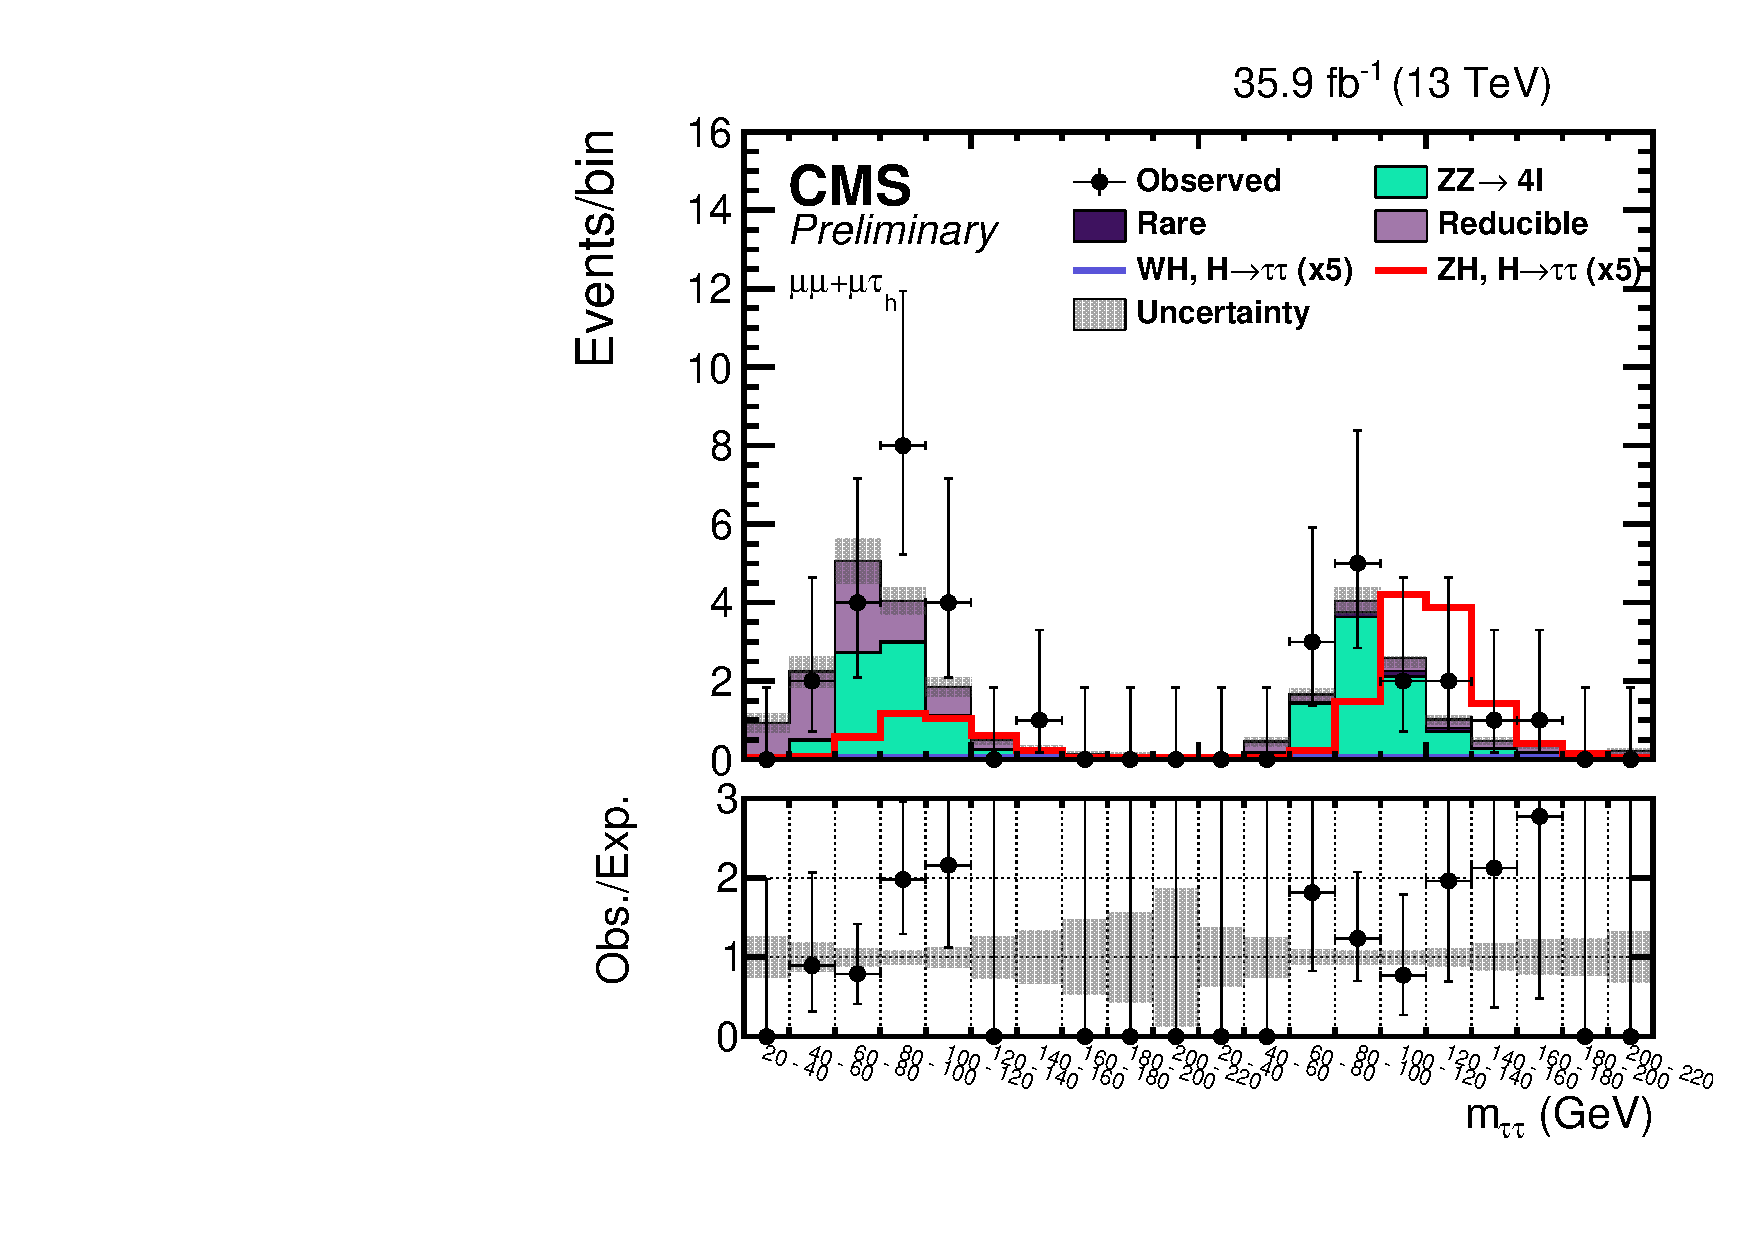
\includegraphics[width=0.45\textwidth]{higgs_to_taus_vh/plots/zh/mmmt_postfit.pdf}
 \end{center}
 \caption{The postfit $\mtt$ distributions used to extract the signal shown
  for the (top left) $\Pe\Pe\Pe\tauh$, (top right) $\Pgm\Pgm\Pe\tauh$, 
  (bottom left) $\Pe\Pe\Pgm\tauh$, and (bottom right) $\Pgm\Pgm\Pgm\tauh$
  final states. The final state is listed in the
  top left corner of each distribution.
  The distributions show full uncertainties.
  The $\PW\PH$ and $\PZ\PH$ signal are shown as 5x larger than their best-fit
  signal strength value of $2.5 \times$ SM.
 }
 \label{fig:zh_all_eight1}
\end{figure}

\begin{figure}[h!]
 \begin{center}
  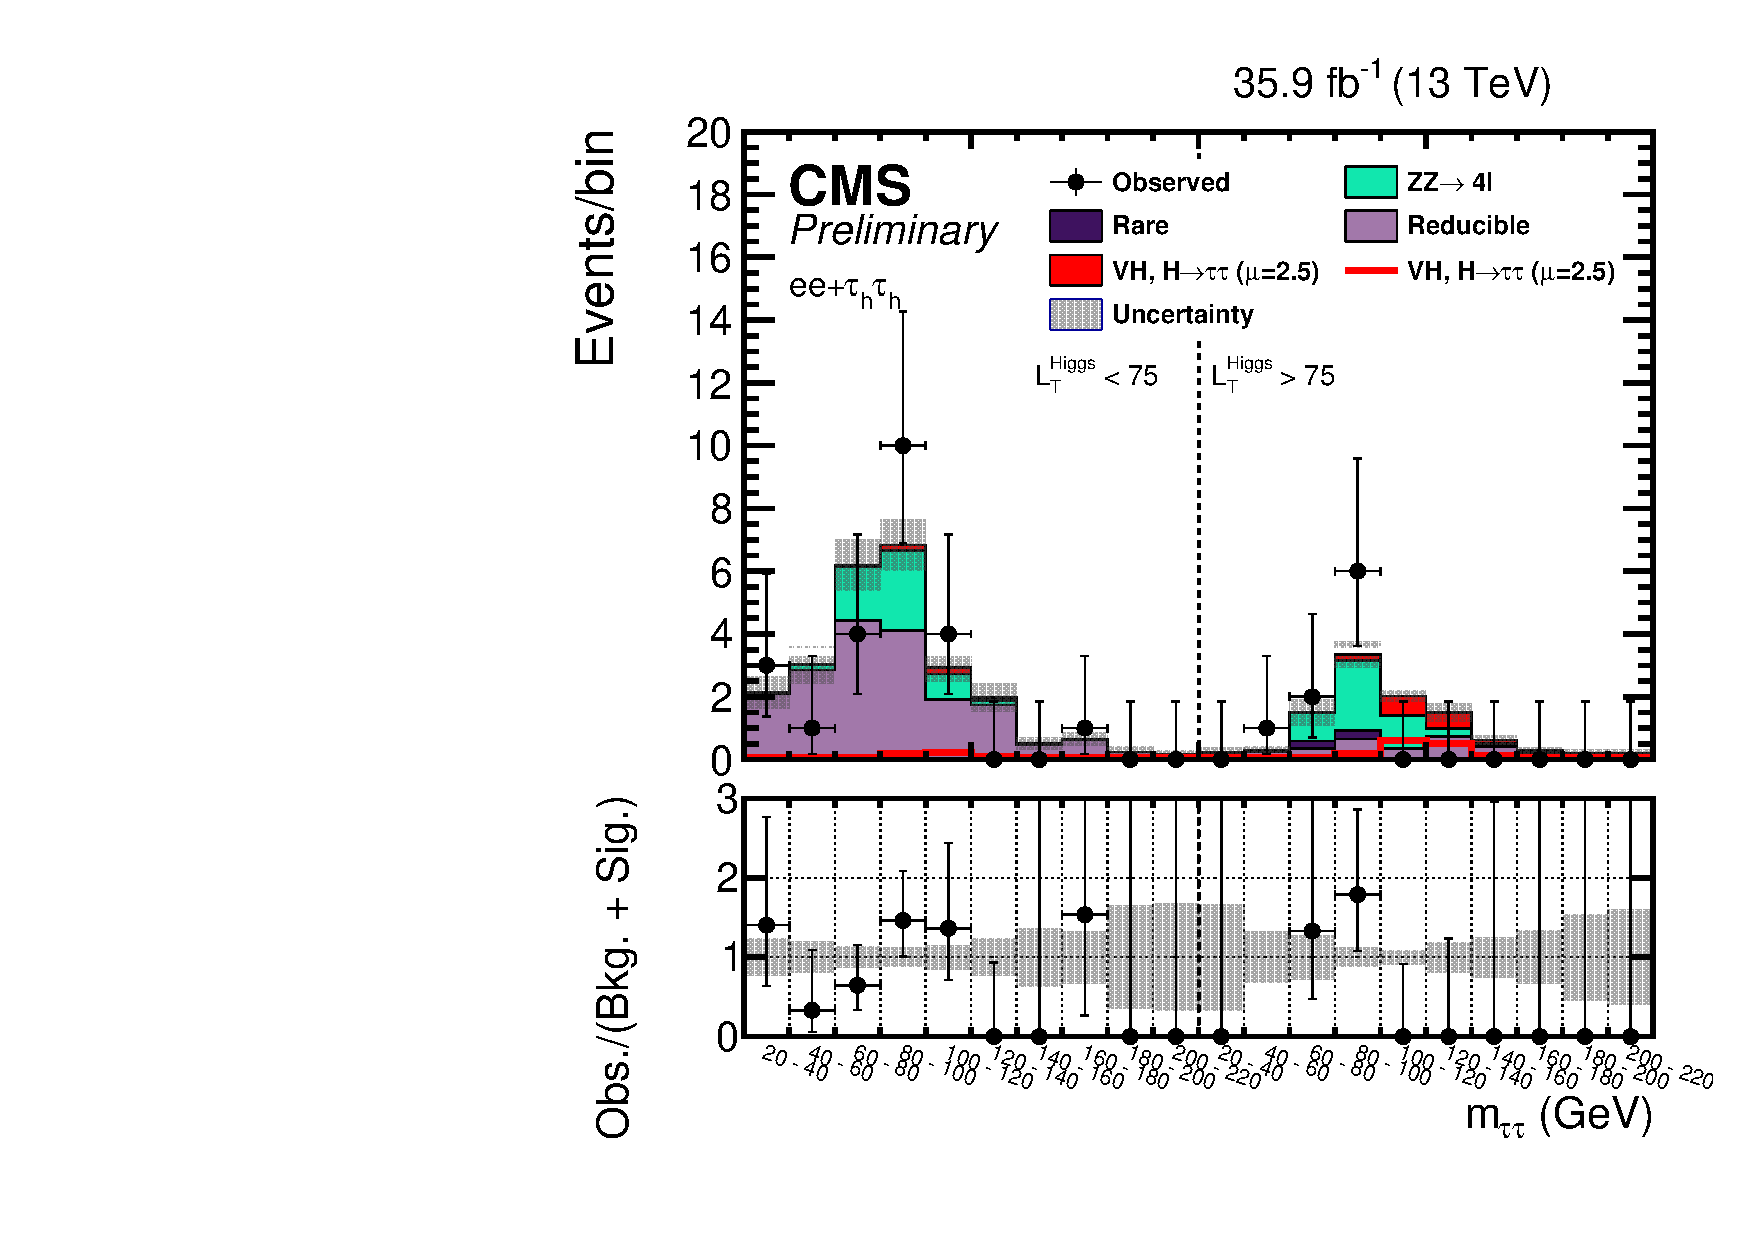
\includegraphics[width=0.45\textwidth]{higgs_to_taus_vh/plots/zh/eett_postfit.pdf}
  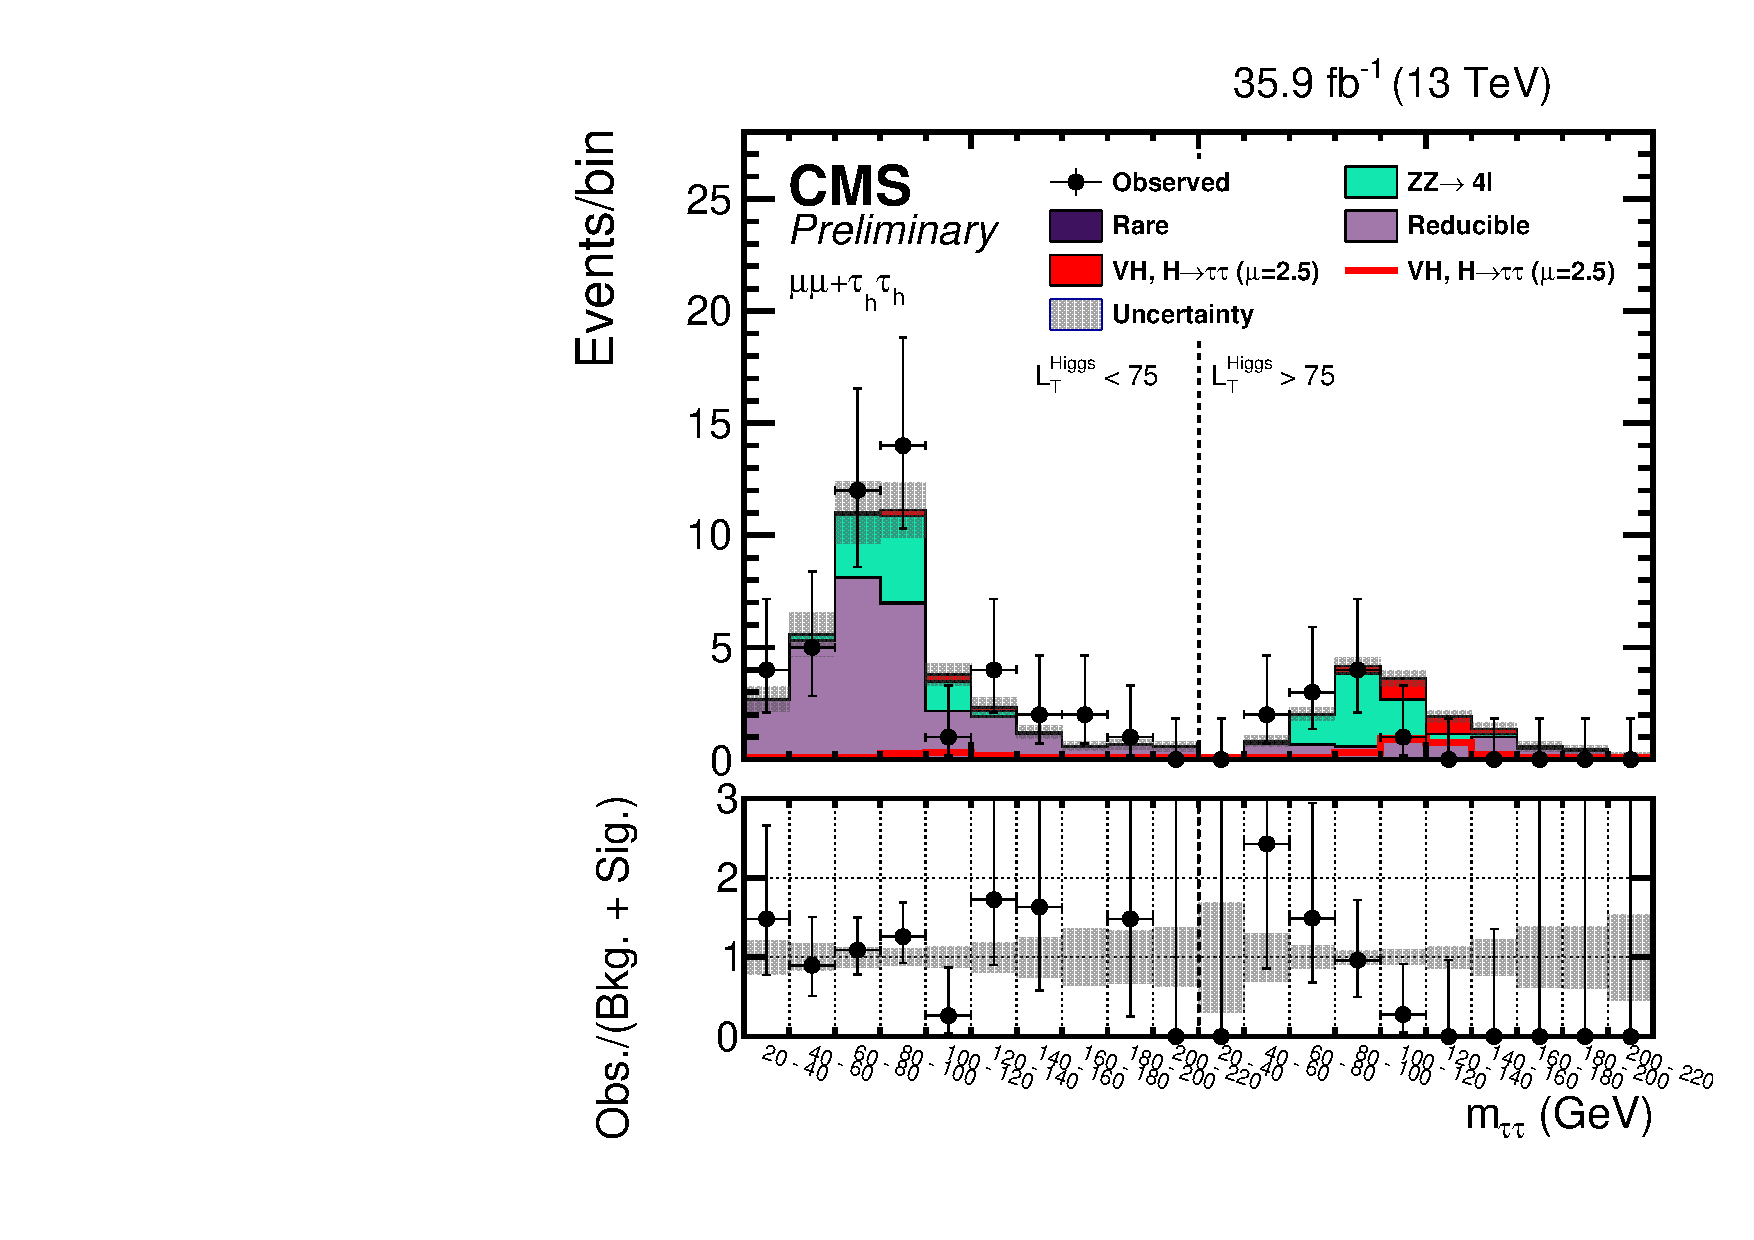
\includegraphics[width=0.45\textwidth]{higgs_to_taus_vh/plots/zh/mmtt_postfit.pdf}
  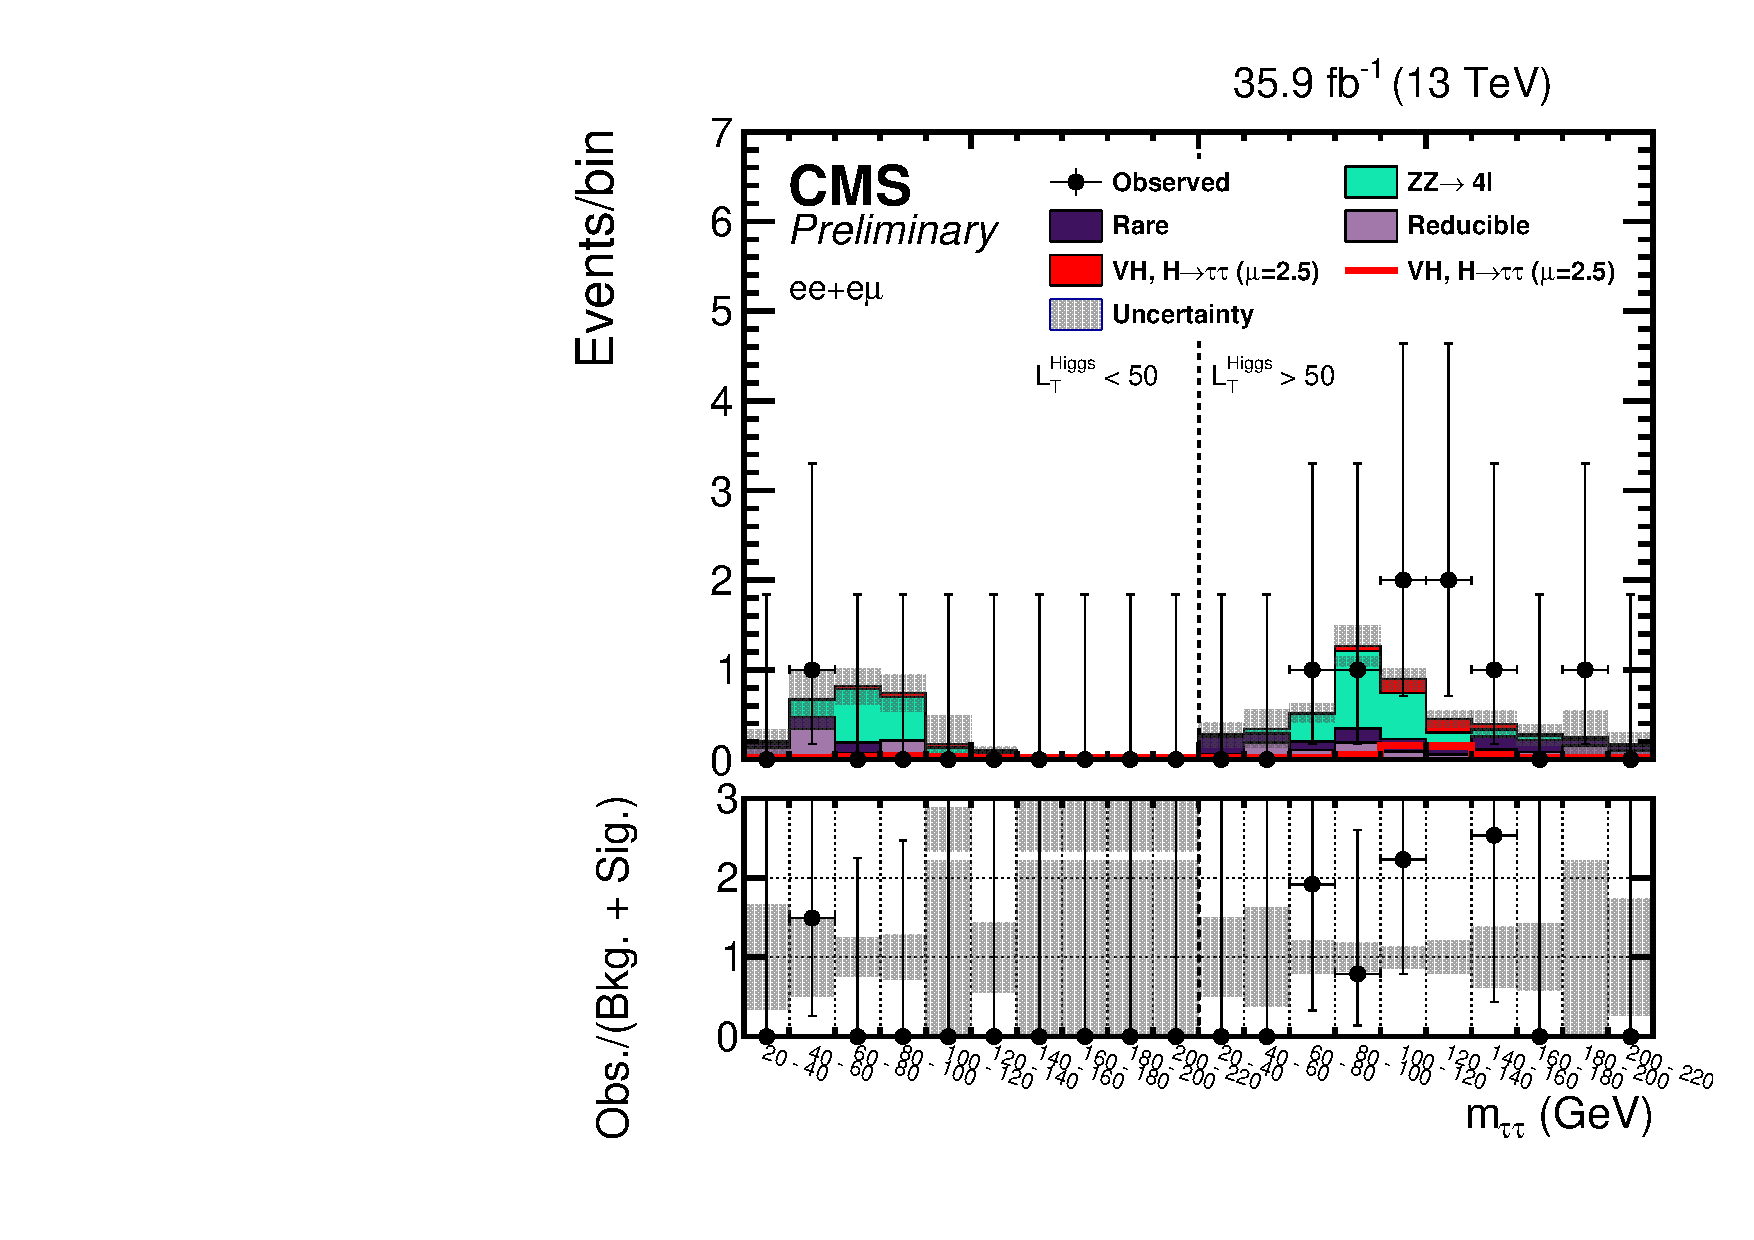
\includegraphics[width=0.45\textwidth]{higgs_to_taus_vh/plots/zh/eeem_postfit.pdf}
  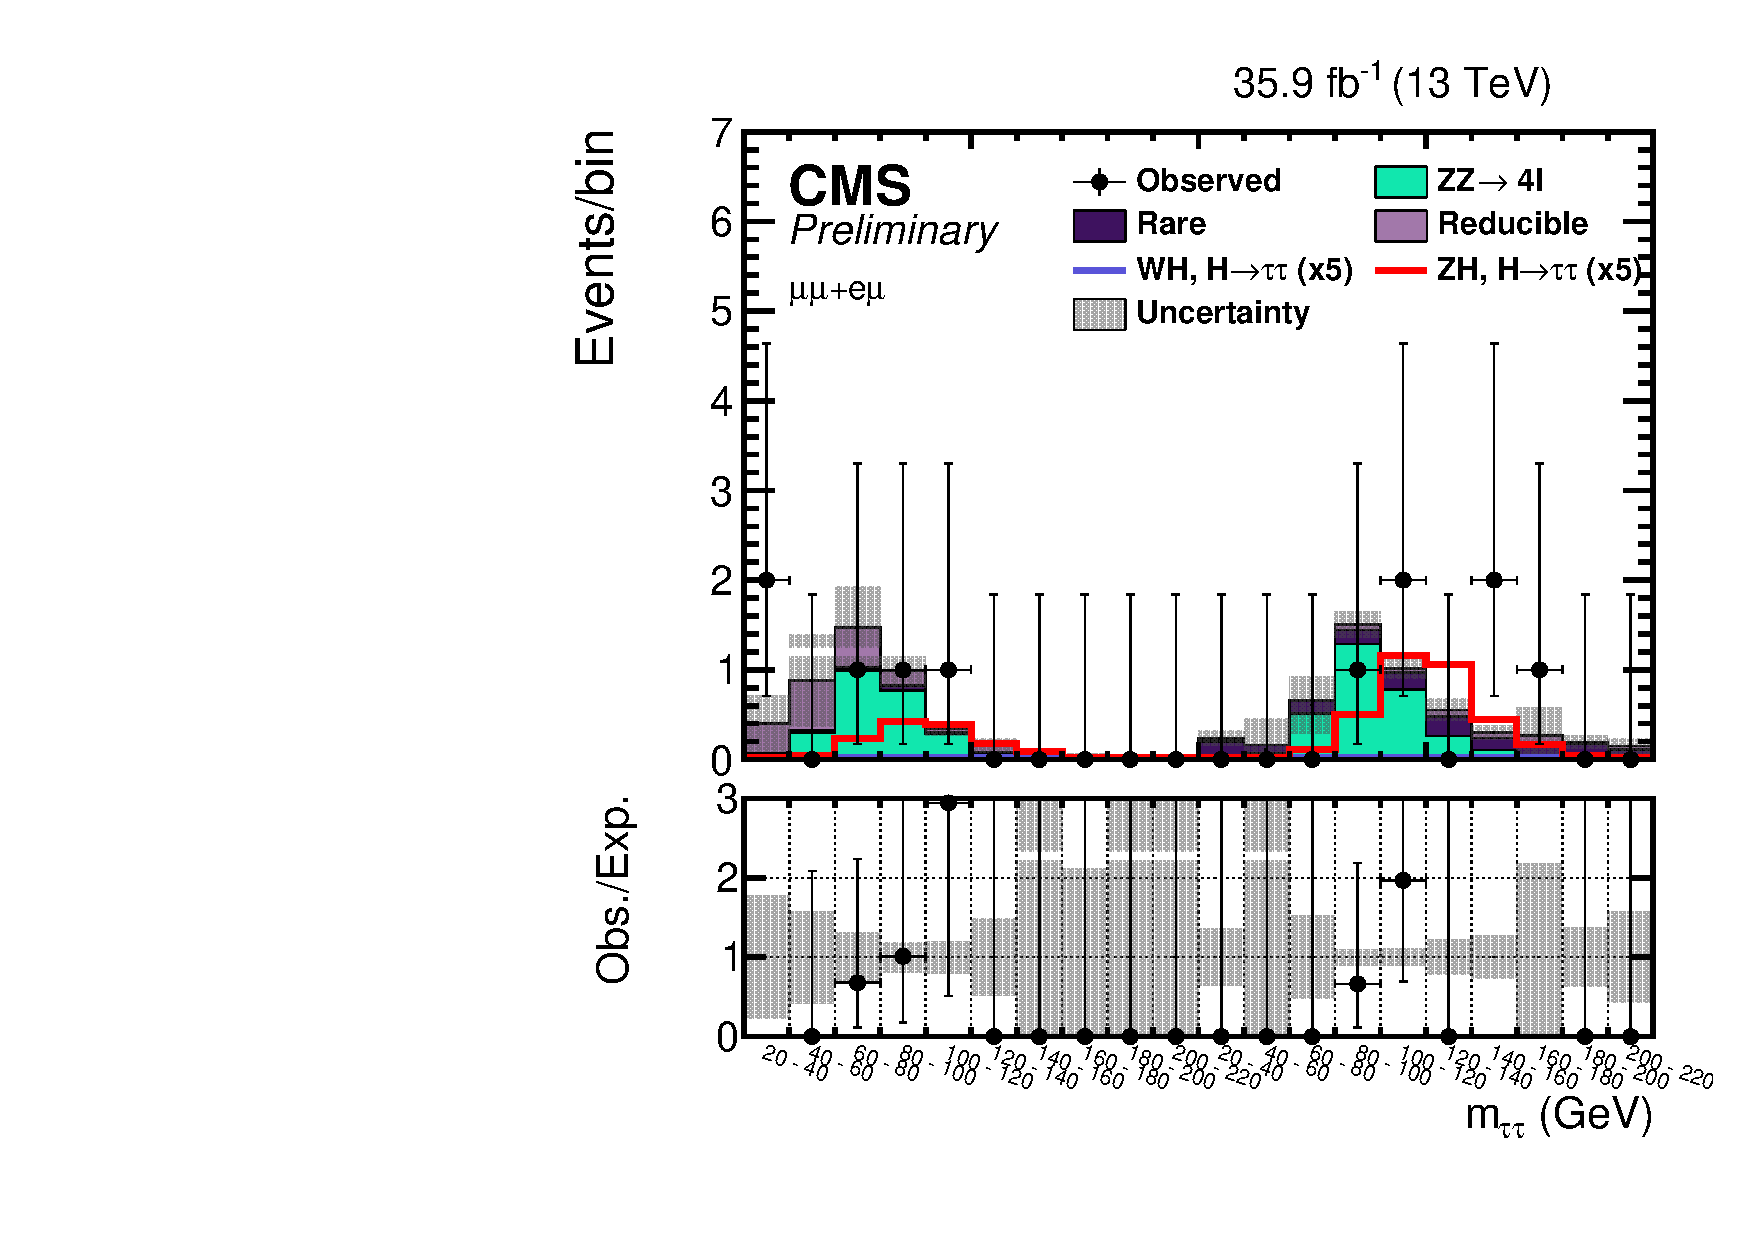
\includegraphics[width=0.45\textwidth]{higgs_to_taus_vh/plots/zh/emmm_postfit.pdf}
 \end{center}
 \caption{The postfit $\mtt$ distributions used to extract the signal shown
  for the (top left) $\Pe\Pe\tauh\tauh$, (top right) $\Pgm\Pgm\tauh\tauh$, 
  (bottom left) $\Pe\Pe\Pe\Pgm$, and (bottom right) $\Pgm\Pgm\Pe\Pgm$
  final states. The final state is listed in the
  top left corner of each distribution.
  The distributions show full uncertainties.
  The $\PW\PH$ and $\PZ\PH$ signal are shown as 5x larger than their best-fit
  signal strength value of $2.5 \times$ SM.
 }
 \label{fig:zh_all_eight2}
\end{figure}

%\begin{figure}[h!]
% \begin{center}
%  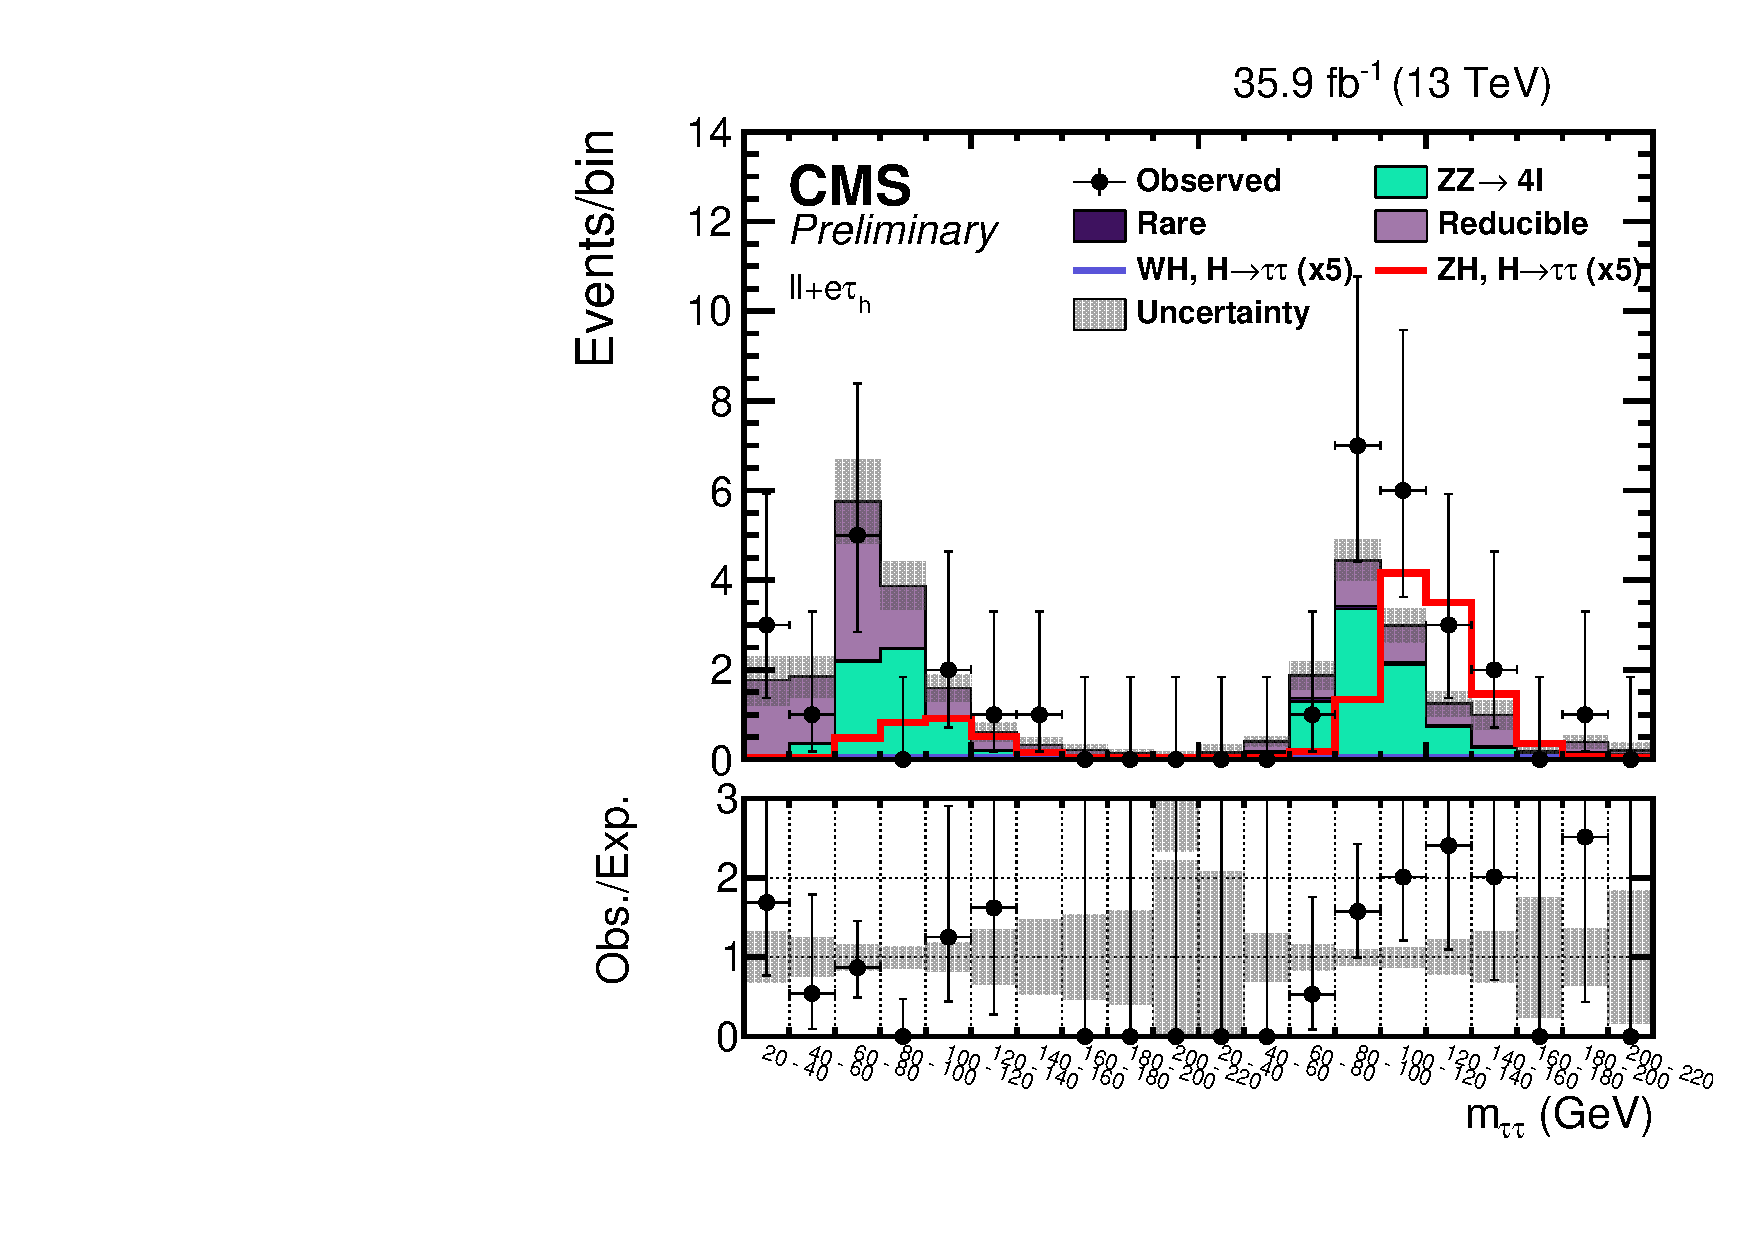
\includegraphics[width=0.45\textwidth]{higgs_to_taus_vh/plots/zh/llet_postfit.pdf}
%  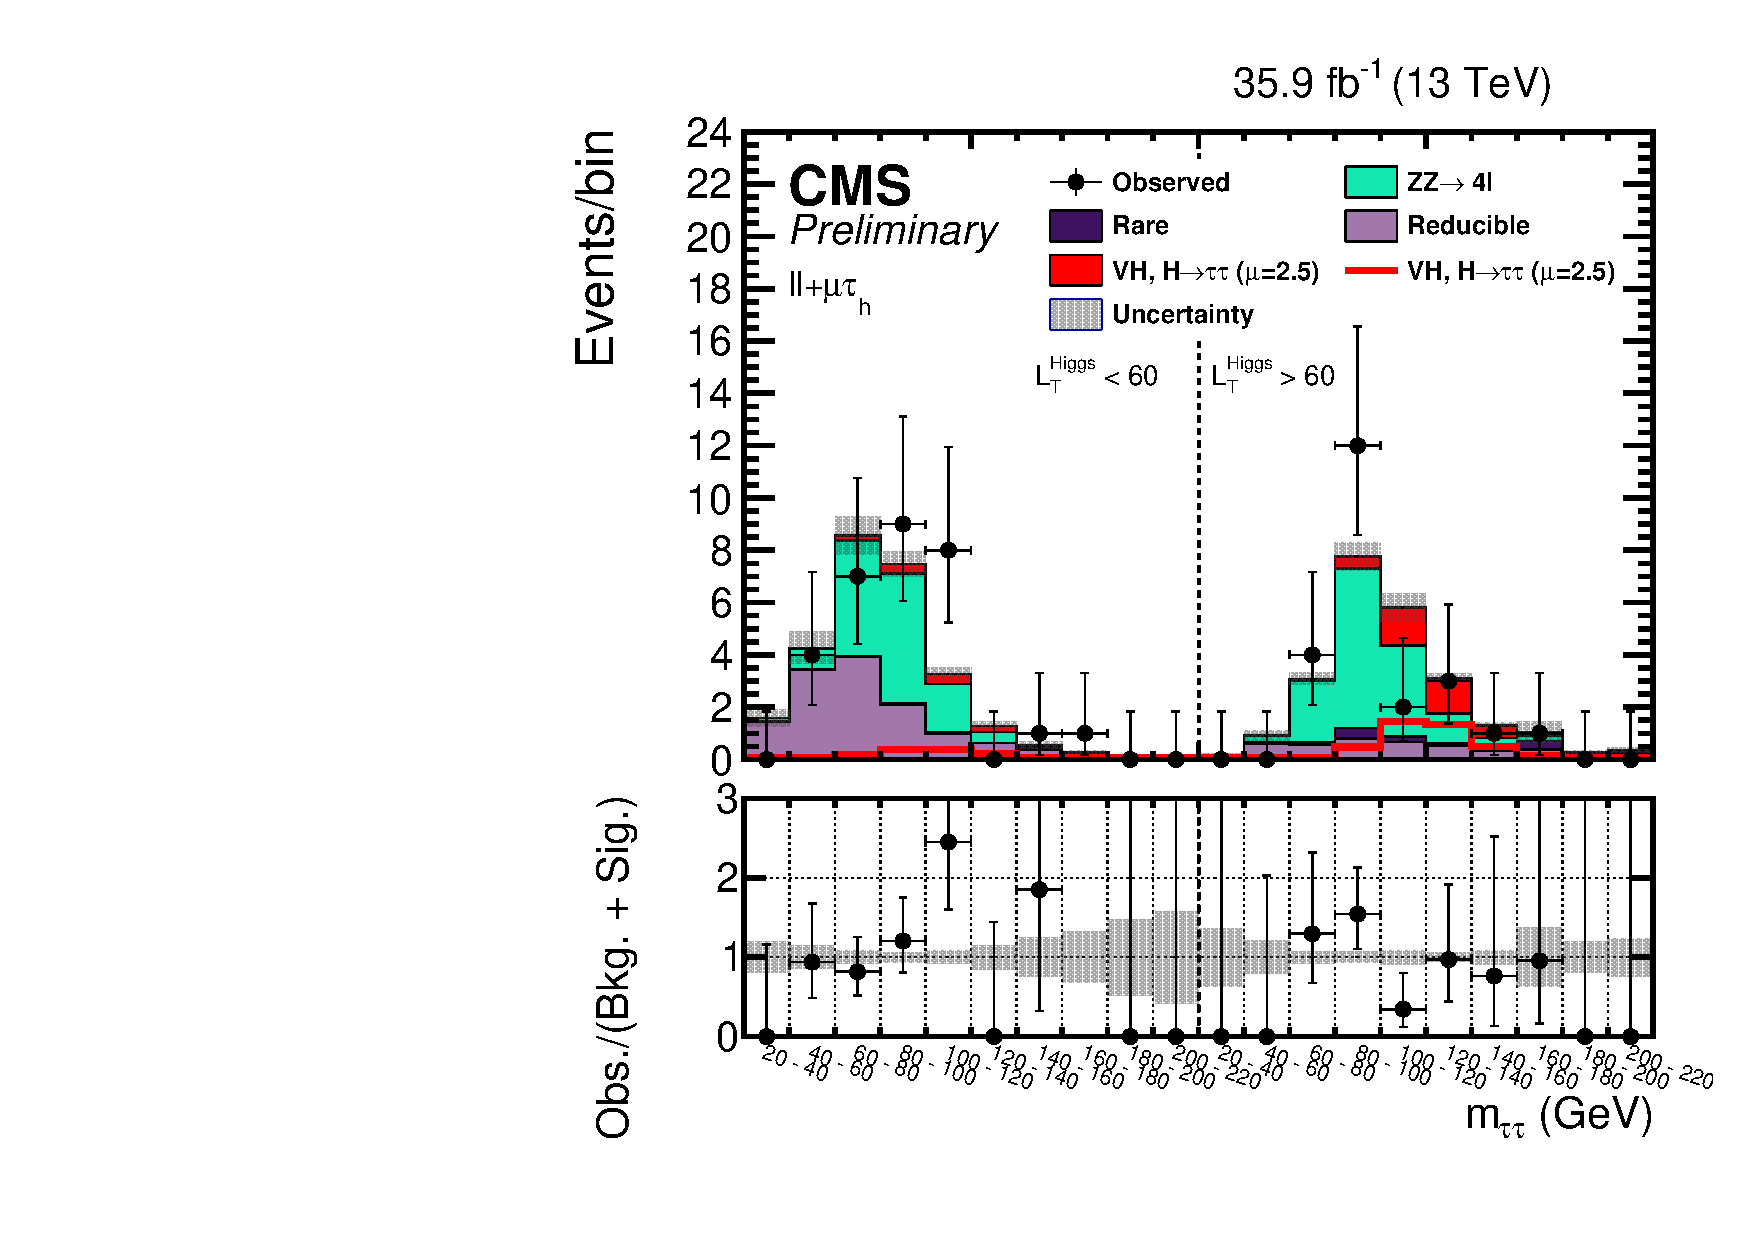
\includegraphics[width=0.45\textwidth]{higgs_to_taus_vh/plots/zh/llmt_postfit.pdf}
%  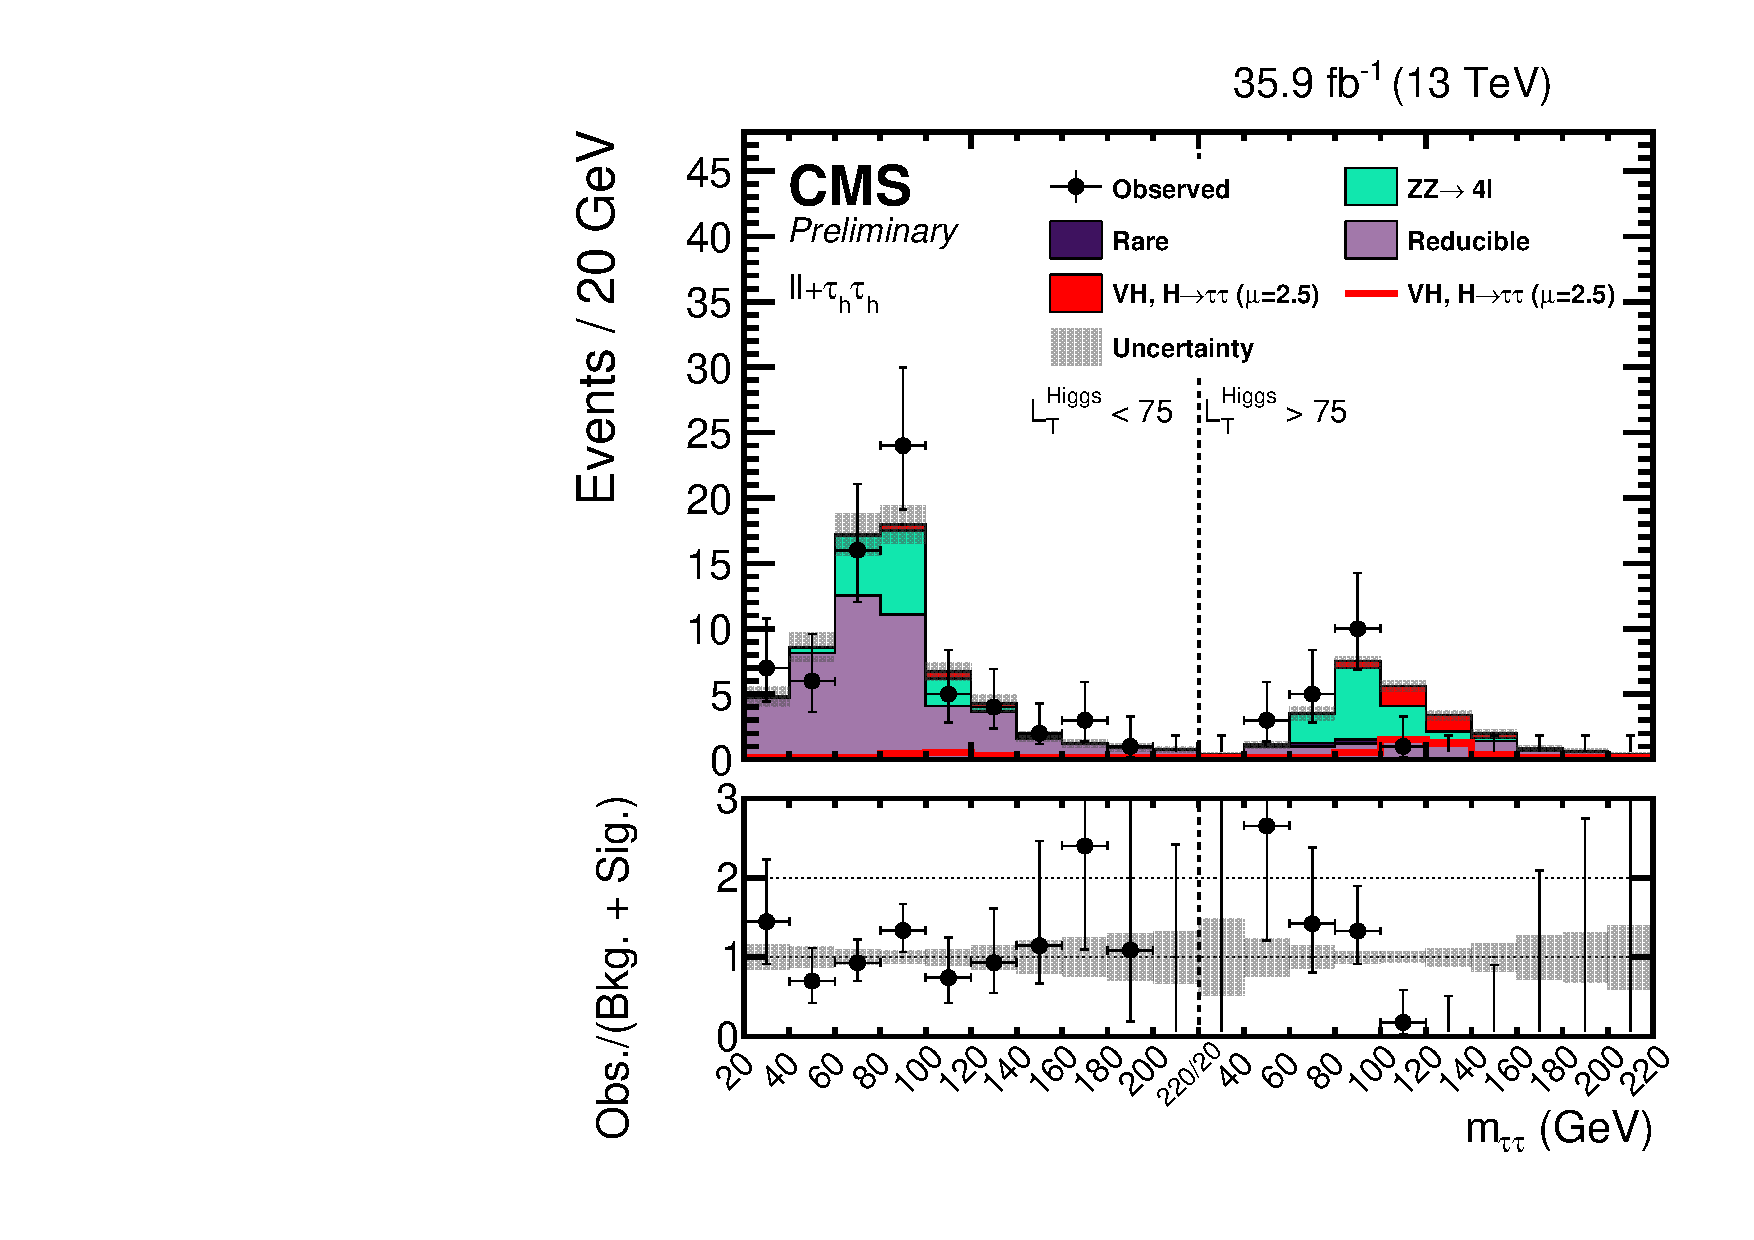
\includegraphics[width=0.45\textwidth]{higgs_to_taus_vh/plots/zh/lltt_postfit.pdf}
%  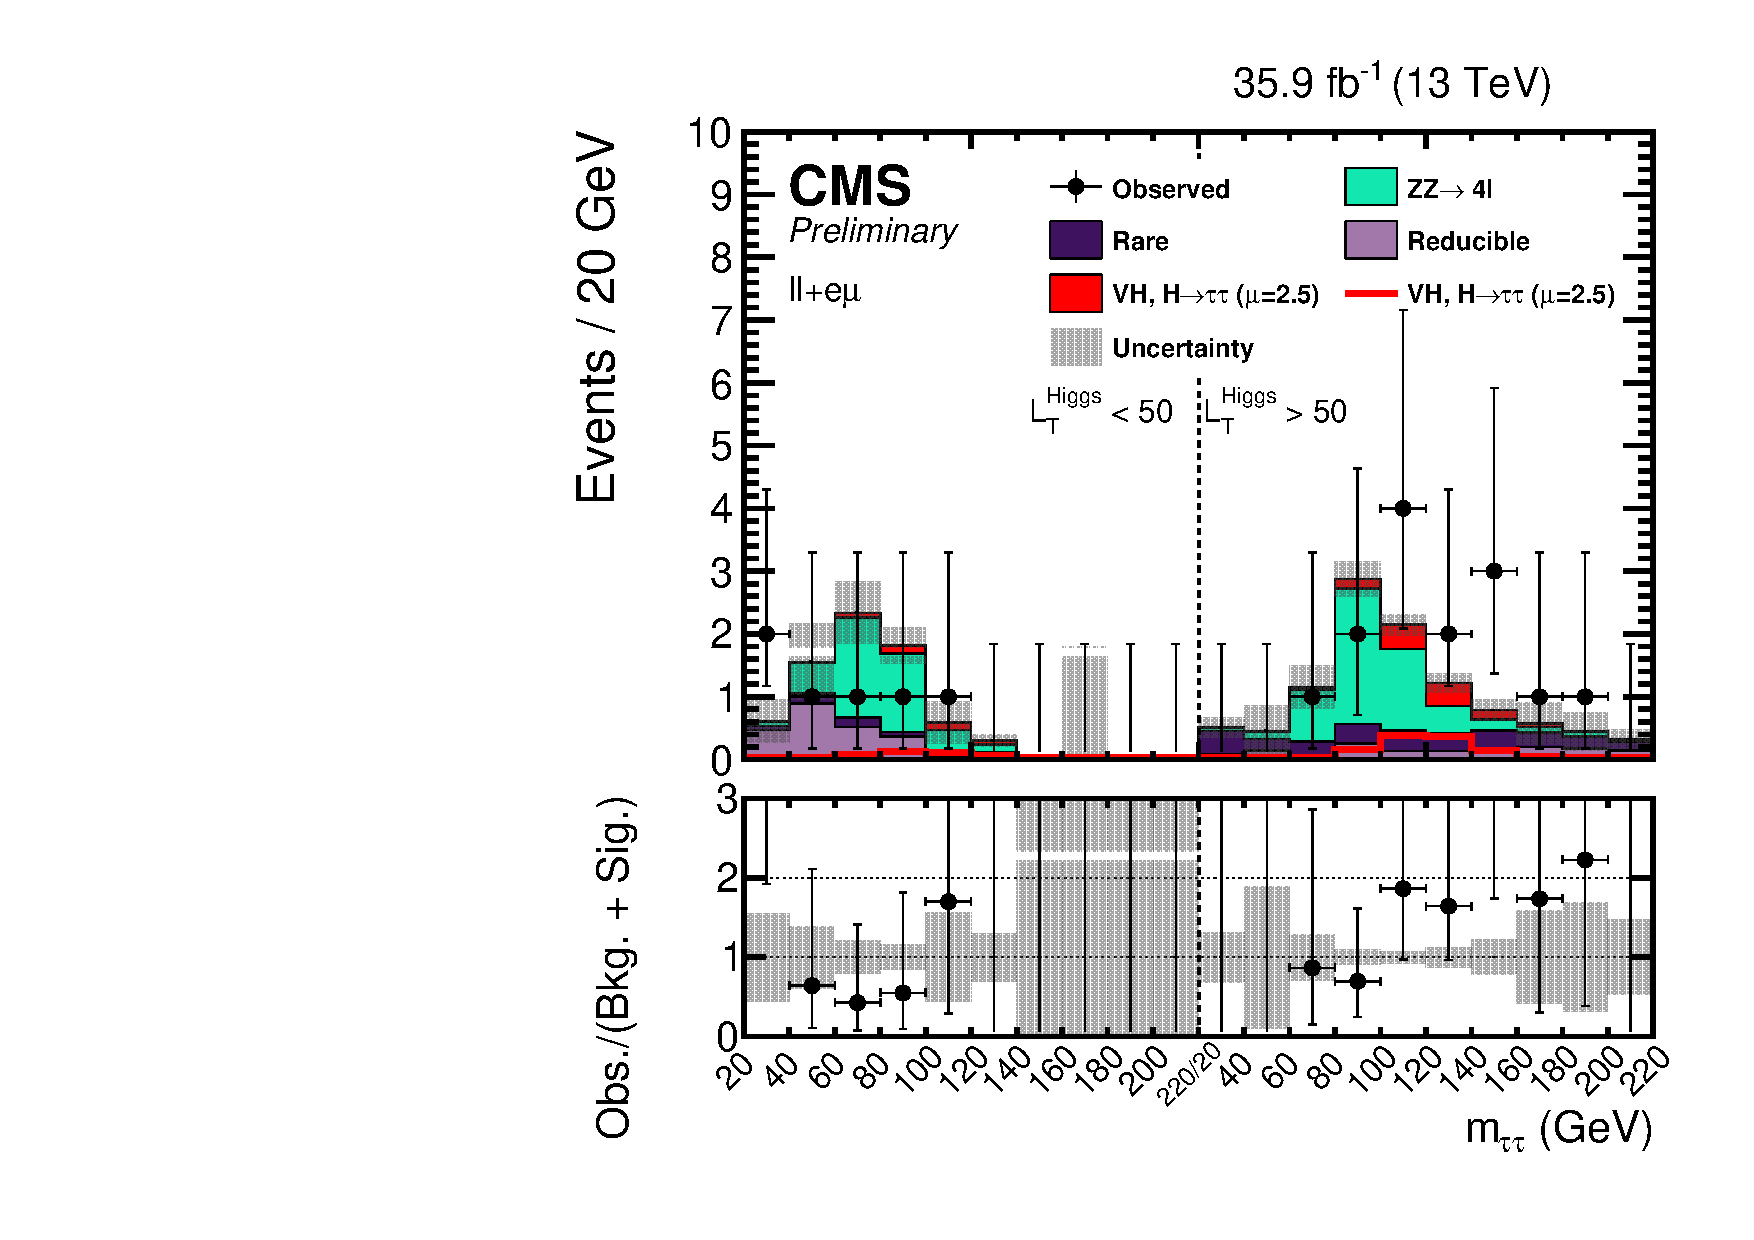
\includegraphics[width=0.45\textwidth]{higgs_to_taus_vh/plots/zh/llem_postfit.pdf}
% \end{center}
% \caption{The postfit $\mtt$ distributions used to extract the signal shown
%  for (top left) $\ell\ell\Pe\tauh$, (top right) $\ell\ell\Pgm\tauh$, 
%  (bottom left) $\ell\ell\tauh\tauh$, and (bottom right) $\ell\ell\Pe\Pgm$.
%  The left half of each distribution is the Low-$L_{T}^{\textrm{Higgs}}$ region
%  while the right half of each distribution is the High--$L_{T}^{\textrm{Higgs}}$ region.
%  $\ell\ell$ covers both $\PZ \to \Pgm\Pgm$ and $\PZ \to \Pe\Pe$ events.
%  The distributions show full uncertainties.
%  The $\PW\PH$ and $\PZ\PH$ signals are shown as 5x larger than their best-fit
%  signal strength value of $2.5 \times$ SM.
% }
% \label{fig:zh_results_svFitLLXX}
%\end{figure}


\begin{figure}[h!]
 \begin{center}
  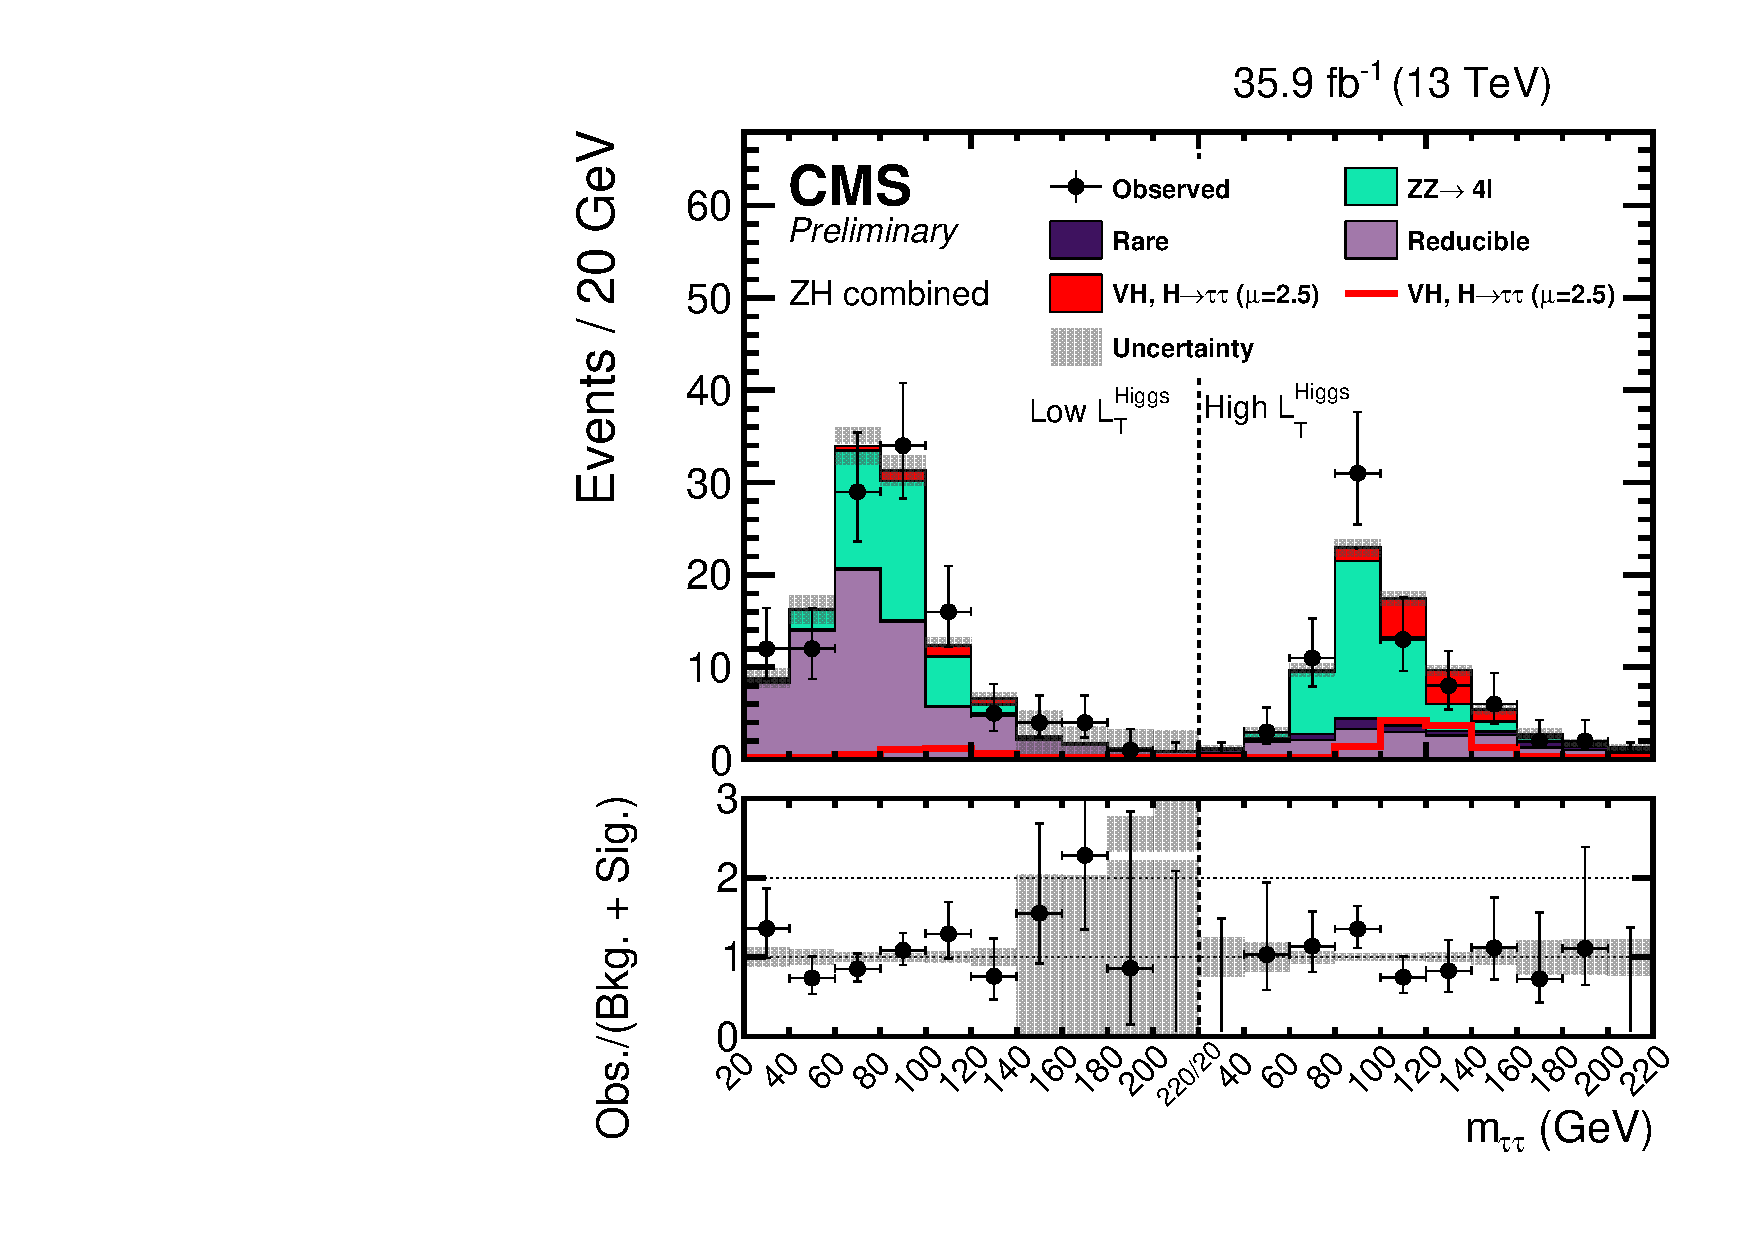
\includegraphics[width=0.65\textwidth]{higgs_to_taus_vh/plots/zh/zh_postfit.pdf}
 \end{center}
 \caption{The postfit $\mtt$ distributions used to extract the signal shown
  for all 8 $\PZ\PH$ channels combined.
  The distribution shows full uncertainties.
  The left half of the distribution is the Low-$L_{T}^{\textrm{Higgs}}$ region
  while the right half corresponds to the High--$L_{T}^{\textrm{Higgs}}$ region.
  The $\PW\PH$ and $\PZ\PH$ signals are shown as 5x larger than their best-fit
  signal strength value of $2.5 \times$ SM.
 }
 \label{fig:zh_results_svFitAll}
\end{figure}

The results in the $\PW\PH$ channels are obtained from the distributions of the 
visible mass of the $\tauh$ candidates in the $\ell\tauh\tauh$ channels, 
and of the visible mass of the $\tauh$ and subleading light lepton in the 
$\ell\ell\tauh$ final states. The mass distributions
are shown in Figs.~\ref{fig:mass_llt} and ~\ref{fig:mass_ltt} for the semileptonic 
and hadronic channels, respectively. Fig.~\ref{fig:mass_wh} shows all
four $\PW\PH$ final states combined together.

\begin{figure}[h!]
 \begin{center}
  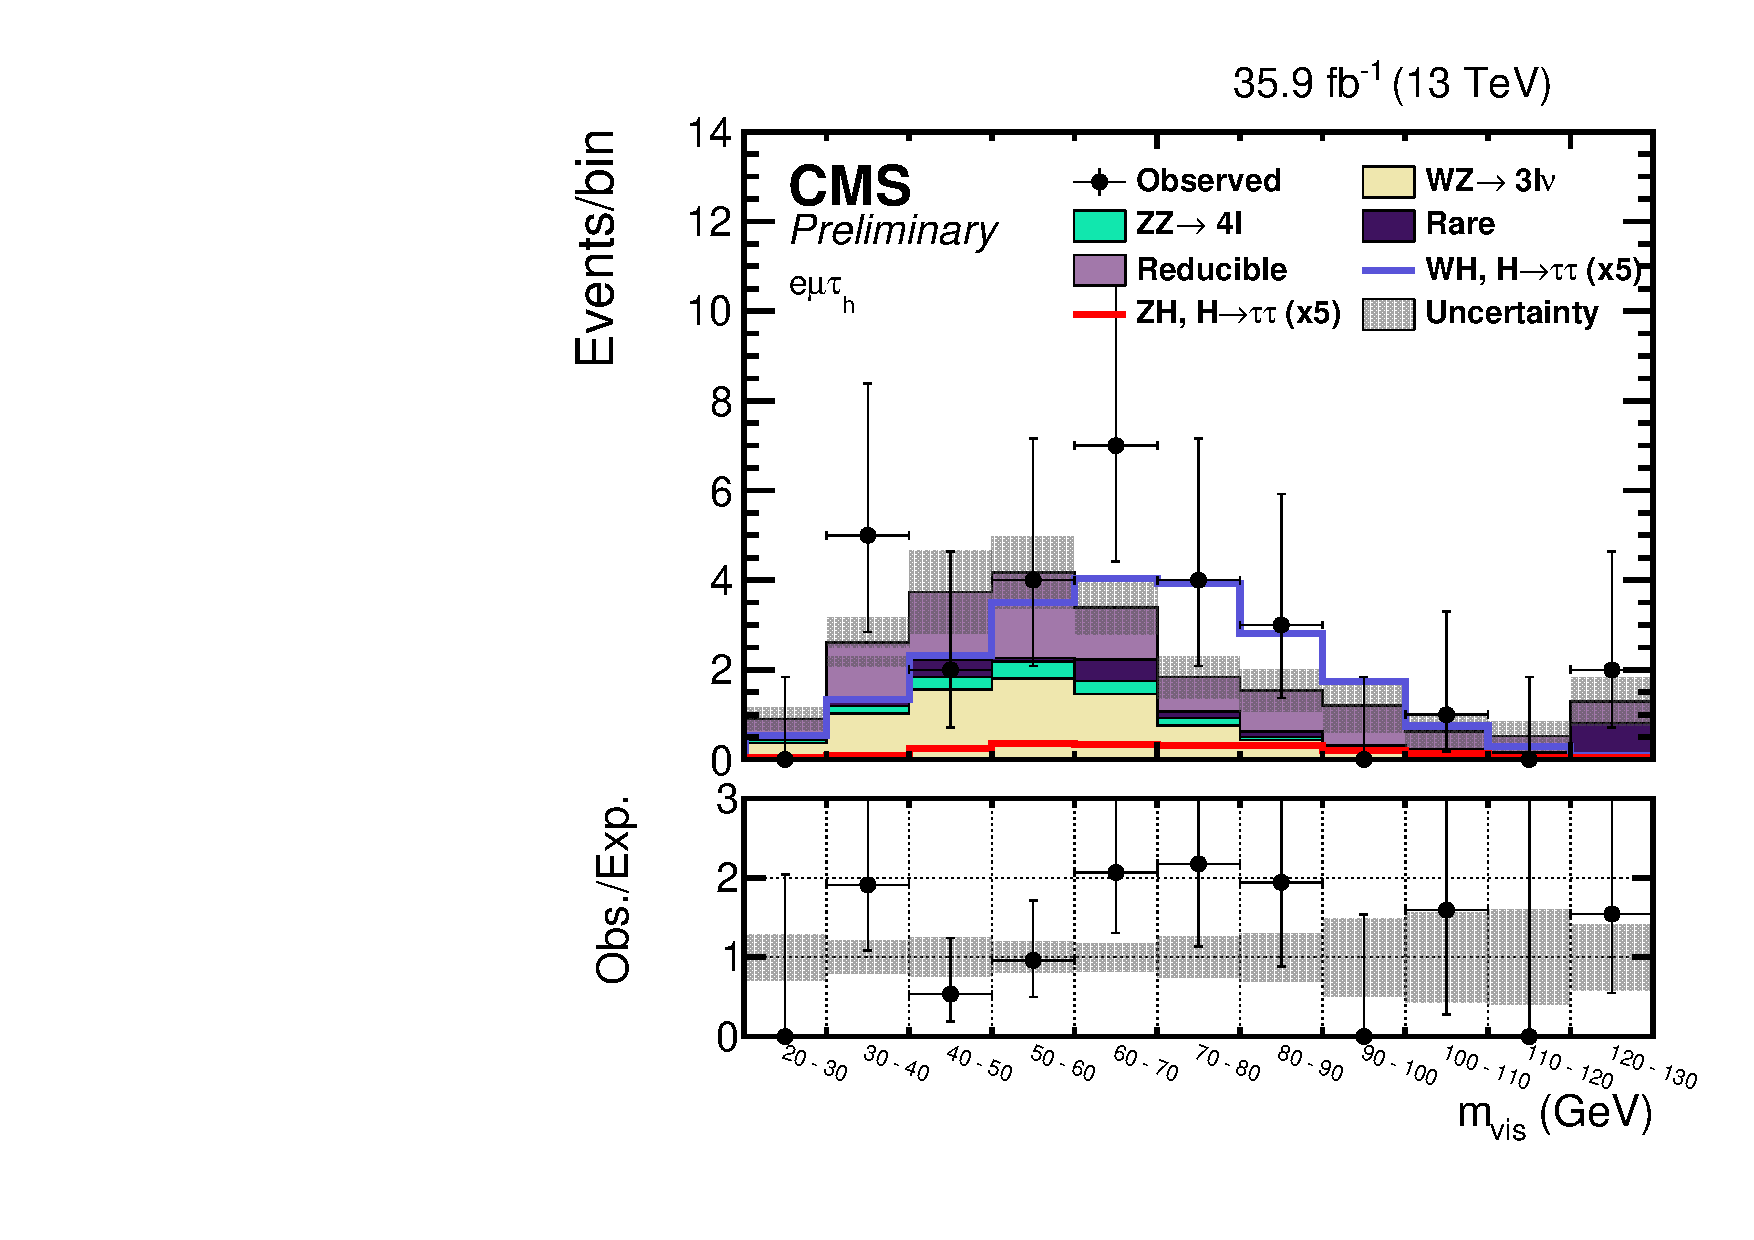
\includegraphics[width=0.45\textwidth]{higgs_to_taus_vh/plots/wh/emt_postfit.pdf}
  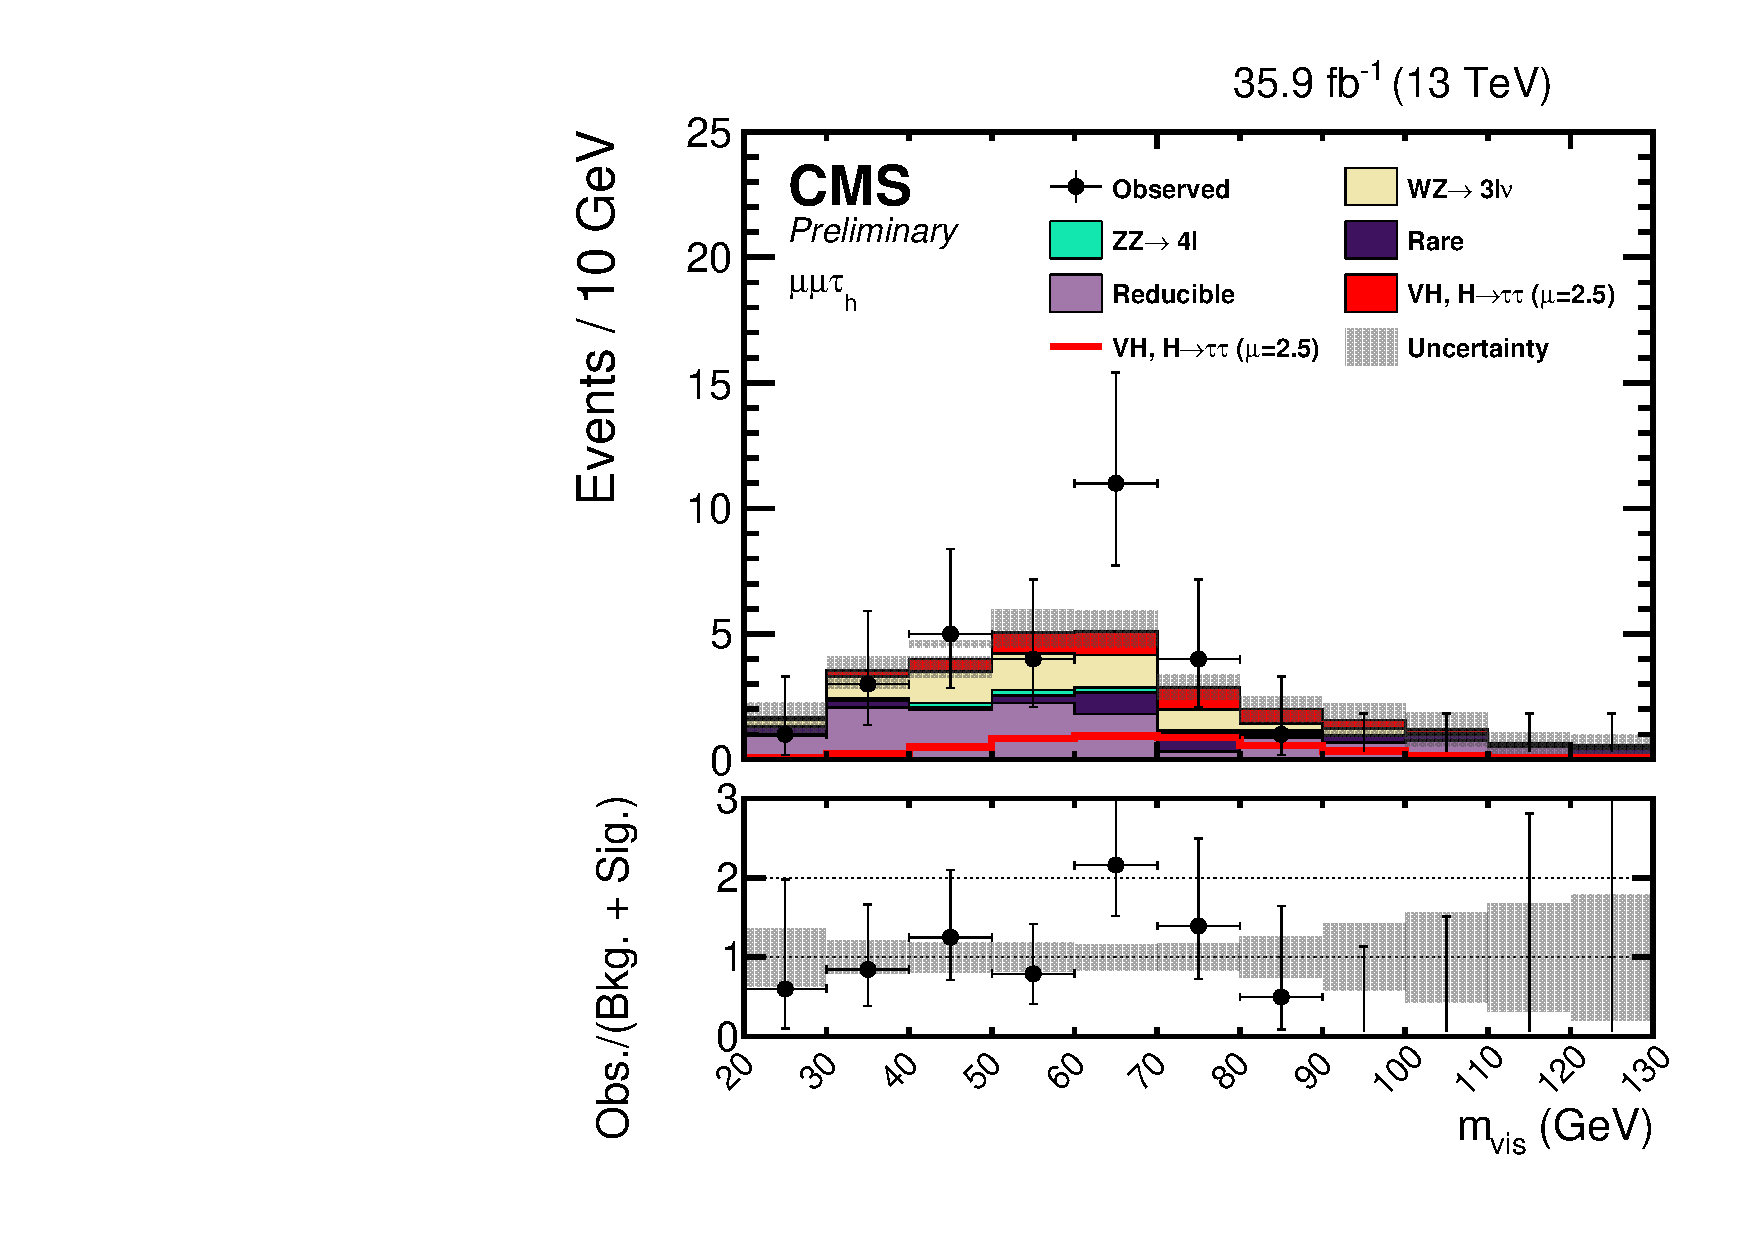
\includegraphics[width=0.45\textwidth]{higgs_to_taus_vh/plots/wh/mmt_postfit.pdf}
 \end{center}
 \caption{Postfit mass distributions in the $\Pe\Pgm\tauh$ (left) and 
 $\Pgm\Pgm\tauh$ (right) final states.
 The distributions show full uncertainties.
 The $\PW\PH$ and $\PZ\PH$ signals are shown as 5x larger than their best-fit
 signal strength value of $2.5 \times$ SM.
 }
 \label{fig:mass_llt}
\end{figure}

\begin{figure}[h!]
 \begin{center}
  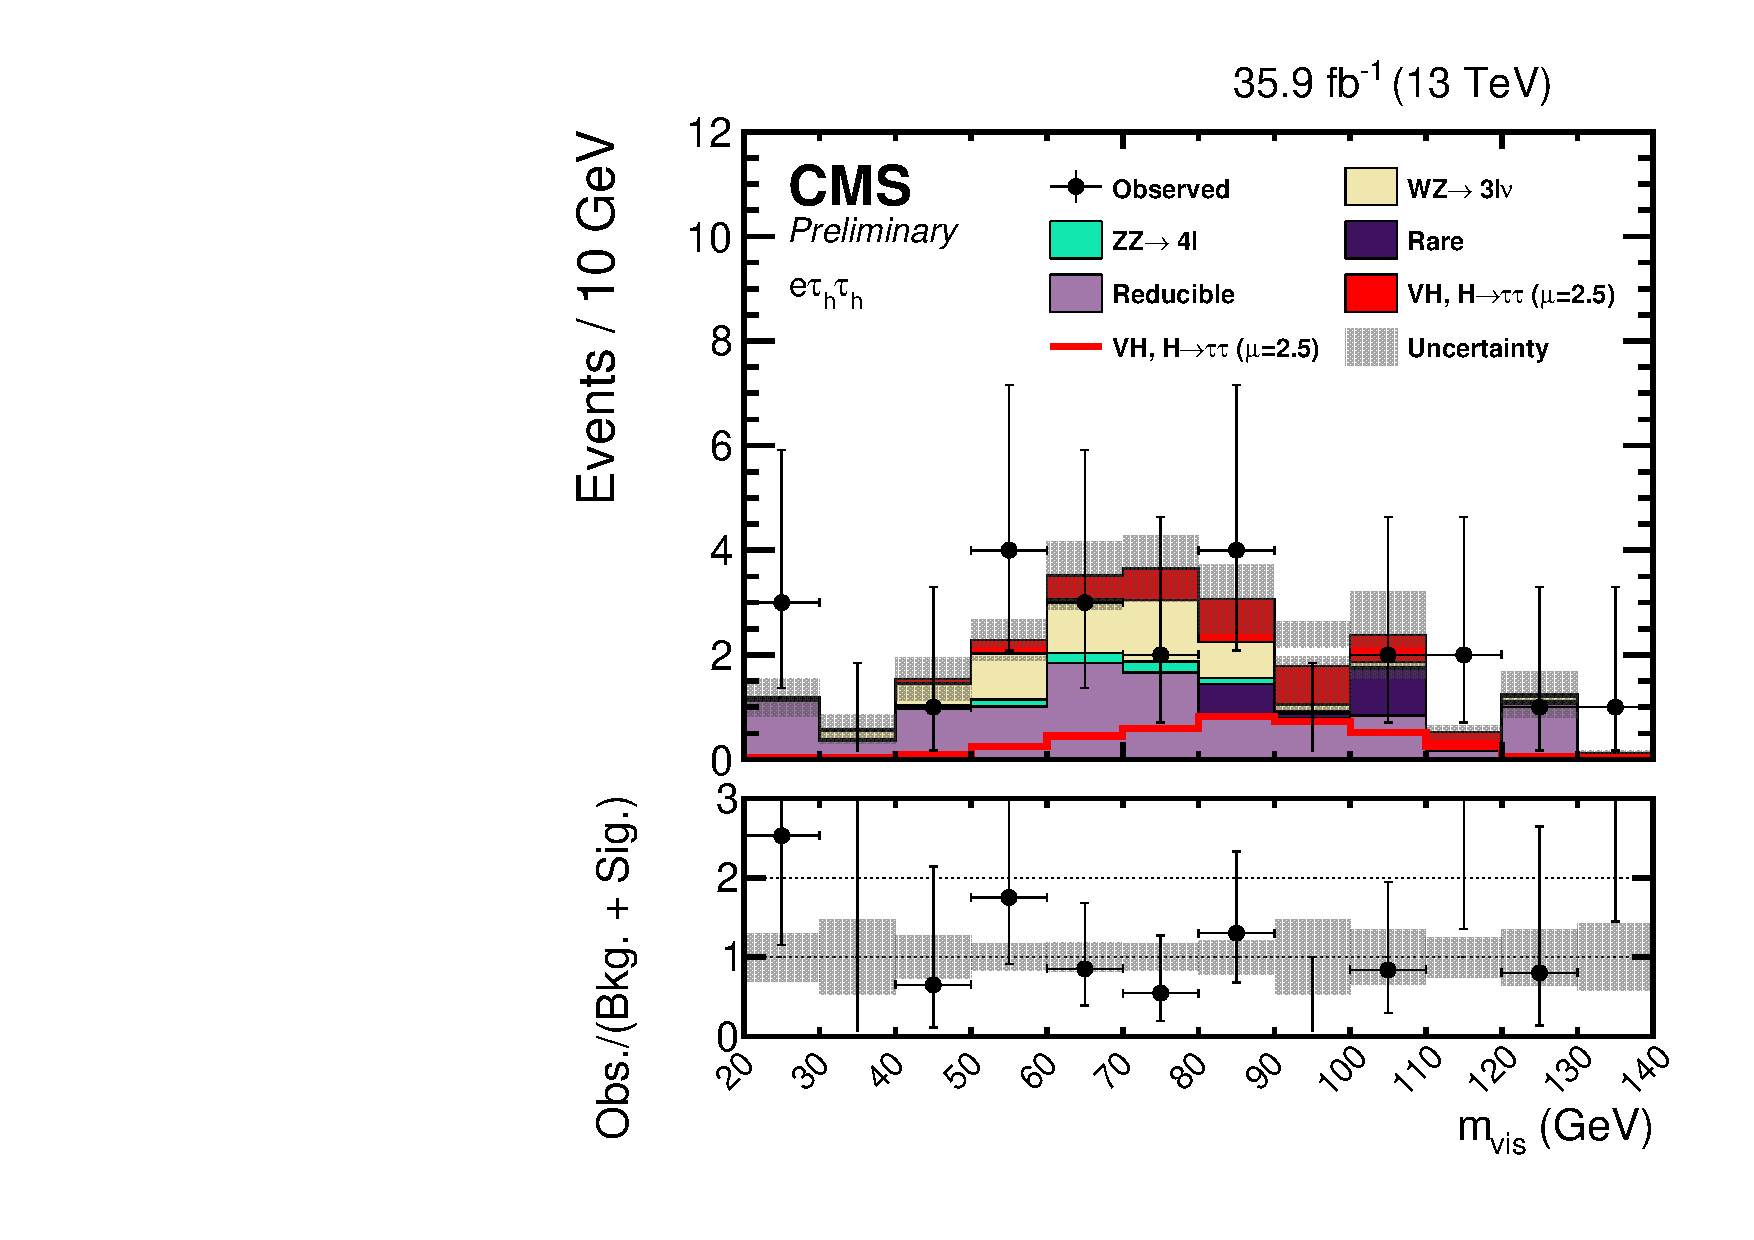
\includegraphics[width=0.45\textwidth]{higgs_to_taus_vh/plots/wh/ett_postfit.pdf}
  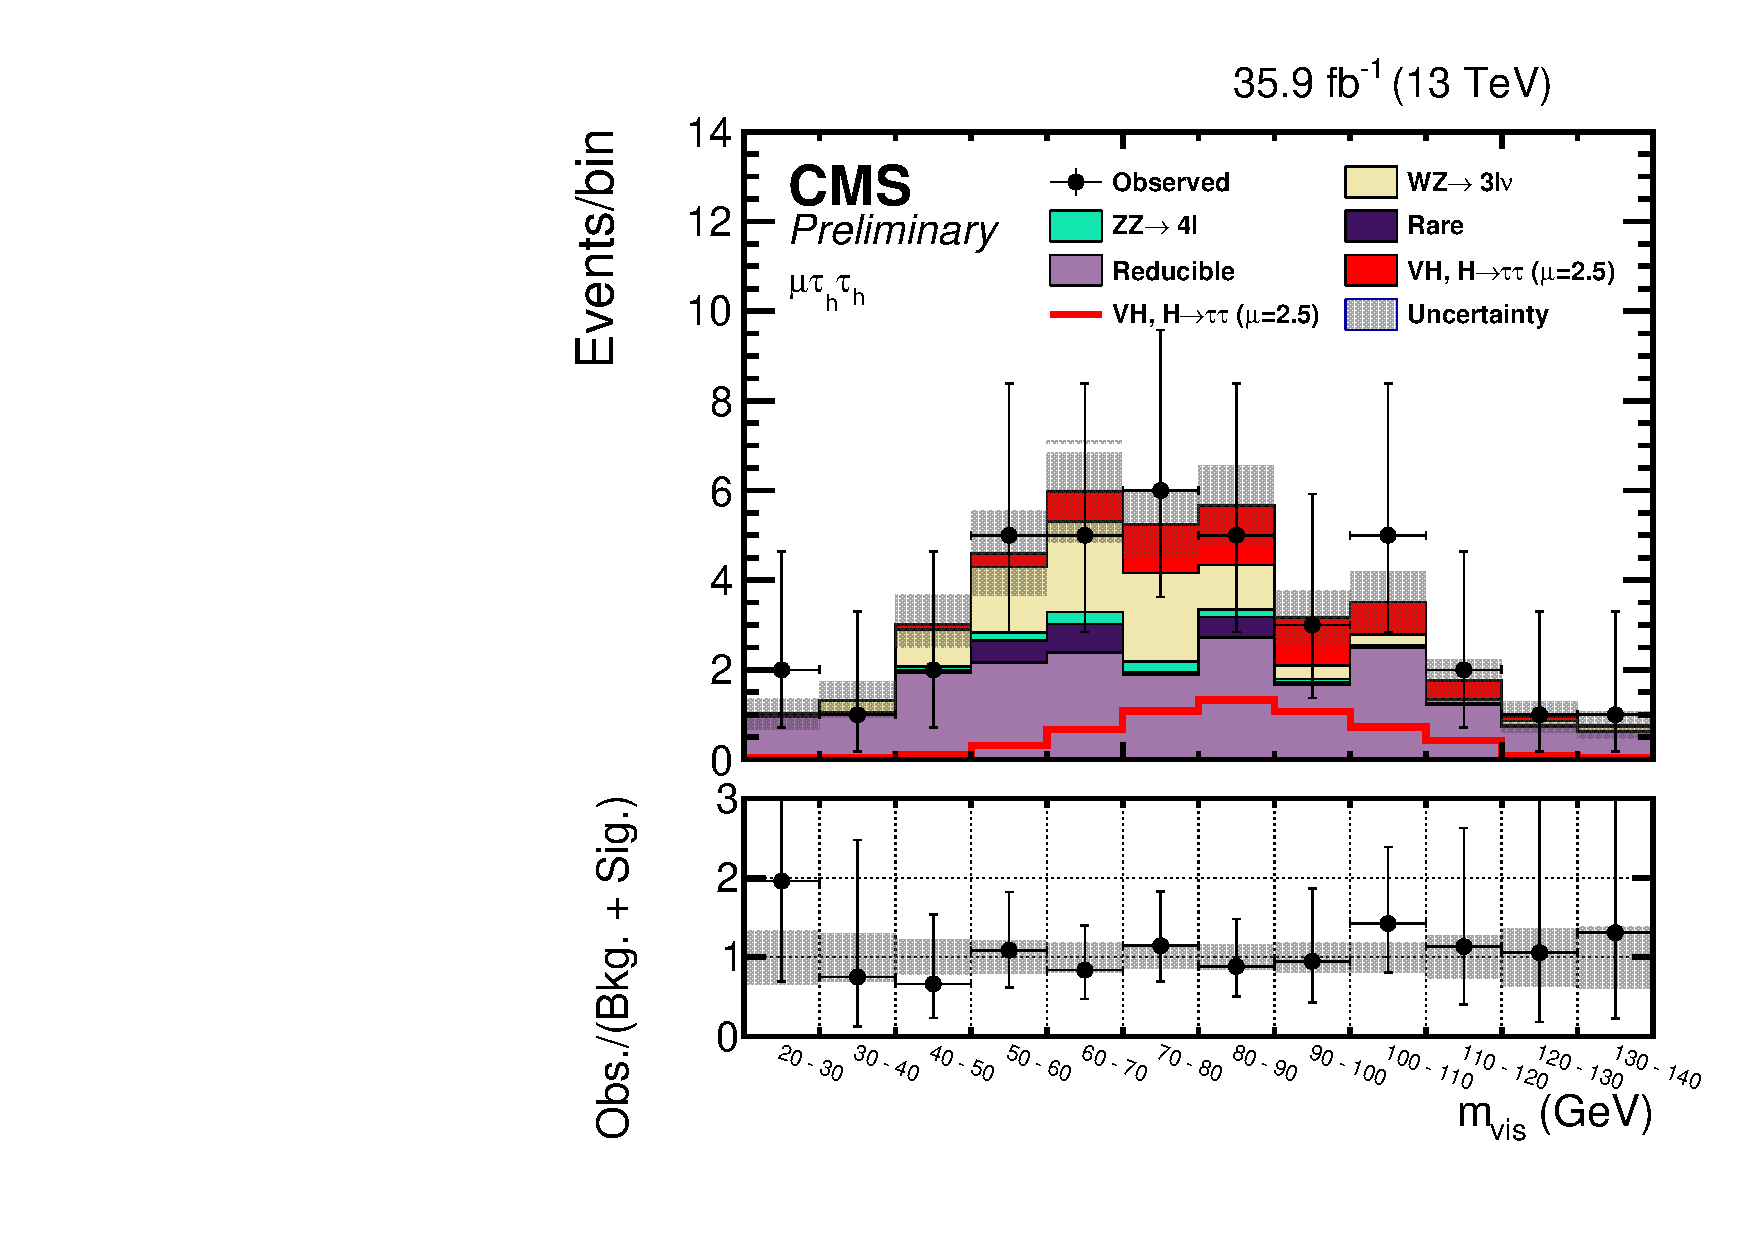
\includegraphics[width=0.45\textwidth]{higgs_to_taus_vh/plots/wh/mtt_postfit.pdf}
 \end{center}
 \caption{Postfit mass distributions in the $\Pe\tauh\tauh$ (left) 
 and $\Pgm\tauh\tauh$ (right) final states.
 The distributions show full uncertainties.
 The $\PW\PH$ and $\PZ\PH$ signals are shown as 5x larger than their best-fit
 signal strength value of $2.5 \times$ SM.
 }
 \label{fig:mass_ltt}
\end{figure}

\begin{figure}[h!]
 \begin{center}
  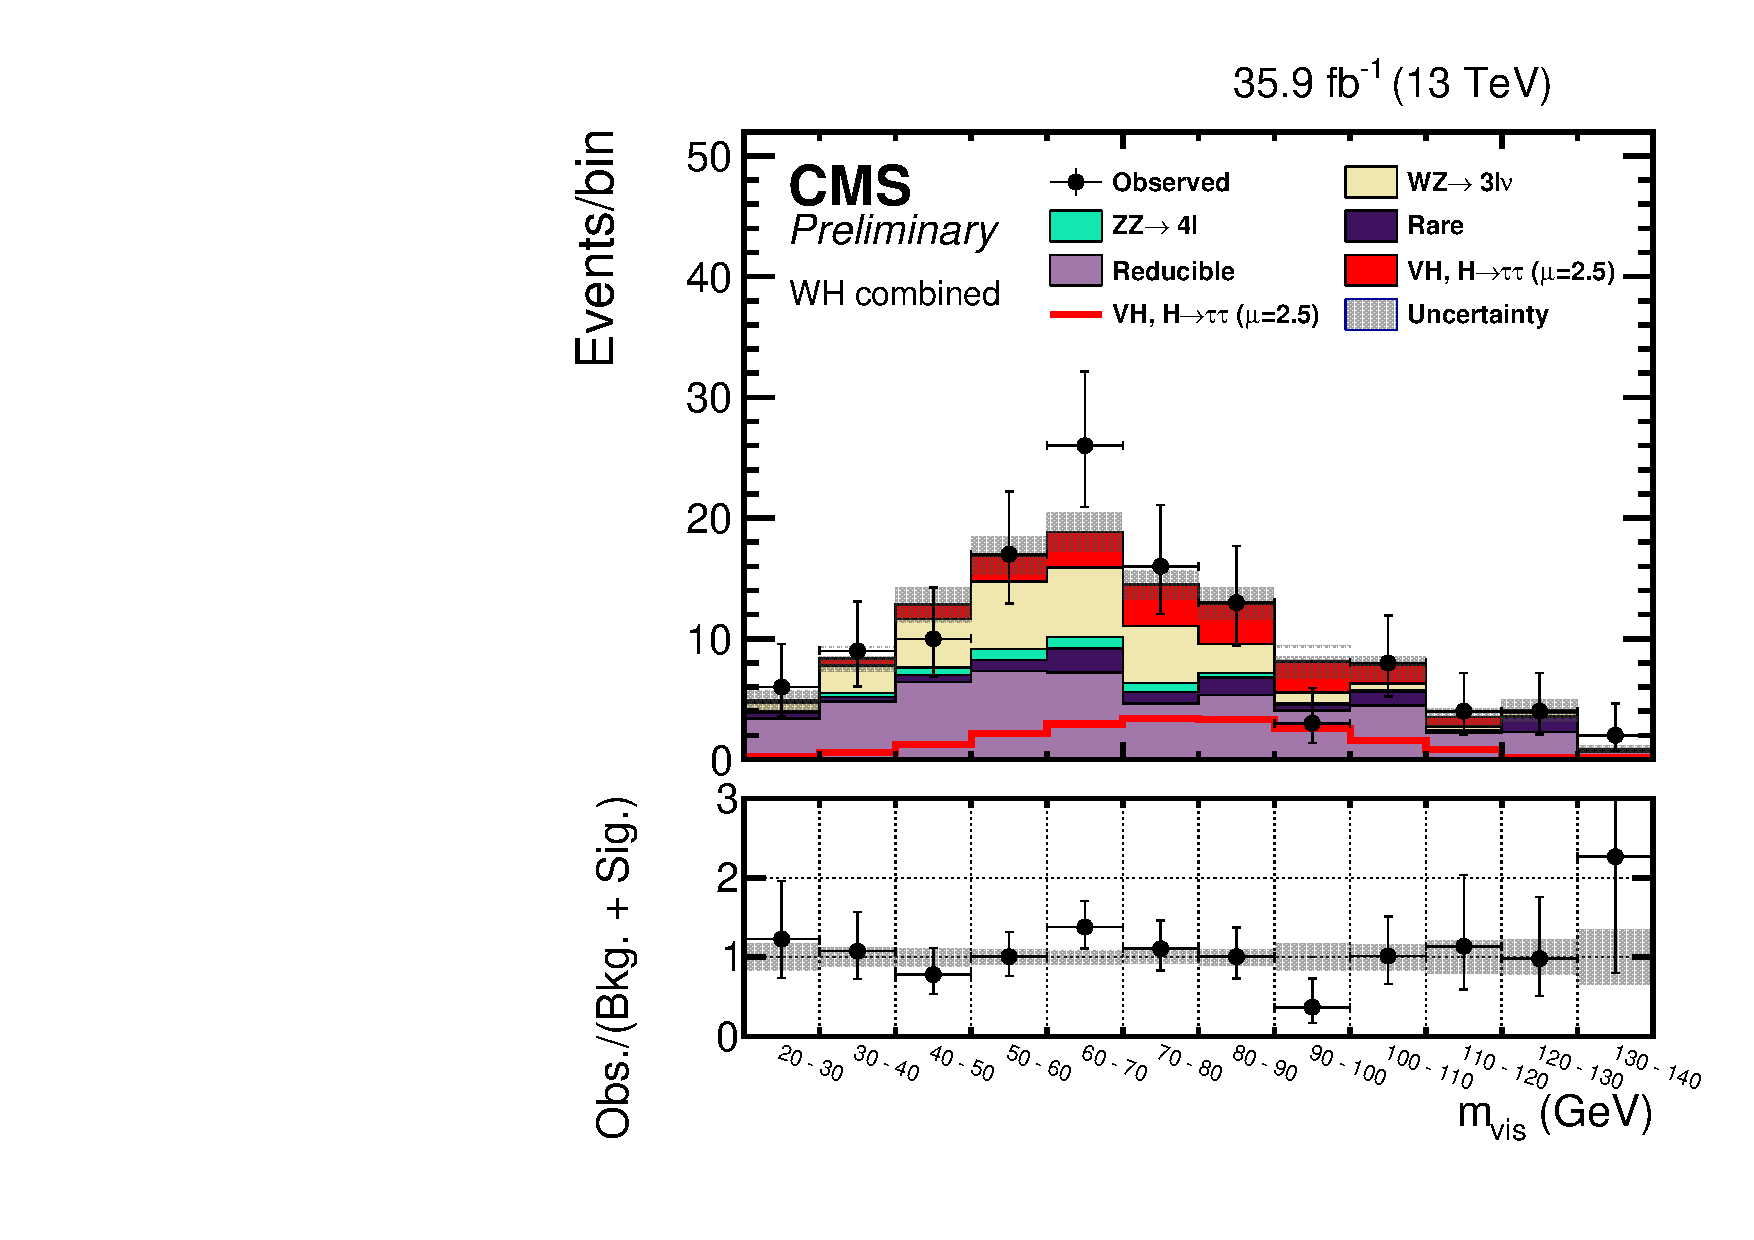
\includegraphics[width=0.65\textwidth]{higgs_to_taus_vh/plots/wh/wh_postfit.pdf}
 \end{center}
 \caption{Postfit mass distributions of the four $\PW\PH$ final states
 combined together. 
 The distributions show full uncertainties.
 The $\PW\PH$ and $\PZ\PH$ signals are shown as 5x larger than their best-fit
 signal strength value of $2.5 \times$ SM.
 }
 \label{fig:mass_wh}
\end{figure}


\begin{table*}
\centering
\begin{small}
\newcolumntype{x}{D{,}{\,\pm\,}{5.5}}
\begin{tabular}{lxxxx}
Process & \multicolumn{1}{c}{$\PW\PH, \Pe\Pgm\tauh$ } & \multicolumn{1}{c}{$\PW\PH, \Pgm\Pgm\tauh$ } & \multicolumn{1}{c}{$\PW\PH, \Pe\tauh\tauh$} & \multicolumn{1}{c}{$\PW\PH, \Pgm\tauh\tauh$}  \\
\hline
$\PZ\PZ$                  & 1.56, 0.05    & 0.93, 0.03  & 0.82, 0.04  & 1.18, 0.05   \\
$\PW\PZ$                  & 7.92, 0.28    & 6.69, 0.24  & 4.83, 0.25  & 8.38, 0.42   \\
Jet Fakes                 & 10.09, 1.61   & 12.19, 1.72 & 10.68, 1.27 & 19.80, 1.87  \\
Rare                      & 2.28, 0.61    & 3.77, 0.84  & 1.71, 1.08  & 1.76, 0.90   \\
Total backgrounds         & 21.85, 1.75   & 23.58, 1.92 & 18.04, 1.67 & 31.12, 2.12  \\
\hline
$\PW\PH, \PH \to\Pgt\Pgt$ & 4.28, 0.72    & 4.25, 0.73  & 3.51, 0.62  &  5.45, 0.97  \\
$\PZ\PH, \PH \to\Pgt\Pgt$ & 0.42, 0.07    & 0.40, 0.08  & 0.33, 0.07  &  0.44, 0.10  \\
Total signal              & 4.70, 0.72    & 4.65, 0.73  & 3.84, 0.92  &  5.98, 0.98  \\
\hline
Observed &  \multicolumn{1}{c}{28 $\pm$ 5.3} &  \multicolumn{1}{c}{29 $\pm$ 5.4} &  \multicolumn{1}{c}{23 $\pm$ 4.8} &  \multicolumn{1}{c}{38 $\pm$ 6.2}  \\
\hline
\end{tabular}
\end{small}
\caption{Background and signal expectations for the $\PW\PH$ channels, 
together with the number of observed 
events, for the post-fit signal region distributions.
$S$ and $B$ are, respectively, the number of expected signal events for a Higgs boson 
with a mass $\mH = 125.09\GeV$ and of expected background events, in those bins. 
The background uncertainty accounts for all sources of background uncertainty, 
systematic as well as statistical, after the global fit. The contribution from 
``Rare'' includes events from triboson, $\ttbar + \PW$/$\PZ$, $\ttbar\PH$ production,
and other rare processes.
}
\label{tab:sb_wh}
\end{table*}

\begin{table*}
\centering
\begin{small}
\newcolumntype{x}{D{,}{\,\pm\,}{5.5}}
\begin{tabular}{lxxxx}
Process & \multicolumn{1}{c}{$\ell\ell\Pe\tauh$} &  \multicolumn{1}{c}{$\ell\ell\Pgm\tauh$} &  \multicolumn{1}{c}{$\ell\ell\tauh\tauh$} &  \multicolumn{1}{c}{$\ell\ell\Pe\Pgm$} \\
\hline
$\PZ\PZ$                        & 14.40, 0.36 & 26.91, 0.55 & 25.58, 1.05 & 9.33, 0.18 \\   
Rare                            & 0.62, 0.08  & 1.54, 0.61  & 0.81, 0.42  & 3.02, 0.23 \\
Jet Fakes                       & 14.01, 1.55 & 17.58, 1.17 & 58.05, 2.87 & 3.66, 4.60 \\
Total backgrounds               & 29.03, 1.59 & 46.03, 1.43 & 84.44, 3.08 & 16.01, 4.61\\             
\hline
$\PW\PH, \PH \to\Pgt\Pgt$       & 0.008, 0.002  & 0.01, 0.003  & 0.016, 0.005  & 0.002, 0.001 \\
$\PZ\PH, \PH \to\Pgt\Pgt$       & 2.83, 0.39  & 5.31, 1.30  & 5.29, 1.17  & 1.62, 0.20 \\
Total signal                    & 2.84, 0.39  & 5.32, 0.70  & 5.31, 1.17  & 1.62, 0.20 \\
\hline
Observed &  \multicolumn{1}{c}{33 $\pm$ 5.75} &  \multicolumn{1}{c}{53 $\pm$ 7.28} &  \multicolumn{1}{c}{87 $\pm$ 9.33} &  \multicolumn{1}{c}{20 $\pm$ 4.47}  \\
\hline
\end{tabular}
\end{small}
\caption{Background and signal expectations for the $\PZ\PH$ channels, 
together with the number of observed 
events, for the post-fit signal region distributions. The $\PZ\PH$ final states
are each grouped according to the Higgs boson decay products. 
$\ell\ell$ covers both $\PZ \to \Pgm\Pgm$ and $\PZ \to \Pe\Pe$ events.
$S$ and $B$ are, respectively, the number of expected signal events for a Higgs boson 
with a mass $\mH = 125.09$\GeV and of expected background events, in those bins. 
The background uncertainty accounts for all sources of background uncertainty, 
systematic as well as statistical, after the global fit. The contribution from 
``Rare'' includes events from triboson, $\ttbar + \PW$/$\PZ$, $\ttbar\PH$ production,
and other rare processes.
}
\label{tab:sb_zh}
\end{table*}


Grouping events in the signal regions by their decimal logarithm of the ratio of the 
signal ($S$) to signal-plus-background ($S+B$) in each bin, Fig.~\ref{fig:sb}, 
an excess of observed events with respect to the SM background expectation is 
visible in the most sensitive bins of the analysis.

\begin{figure}[!ht]
 \begin{center}
  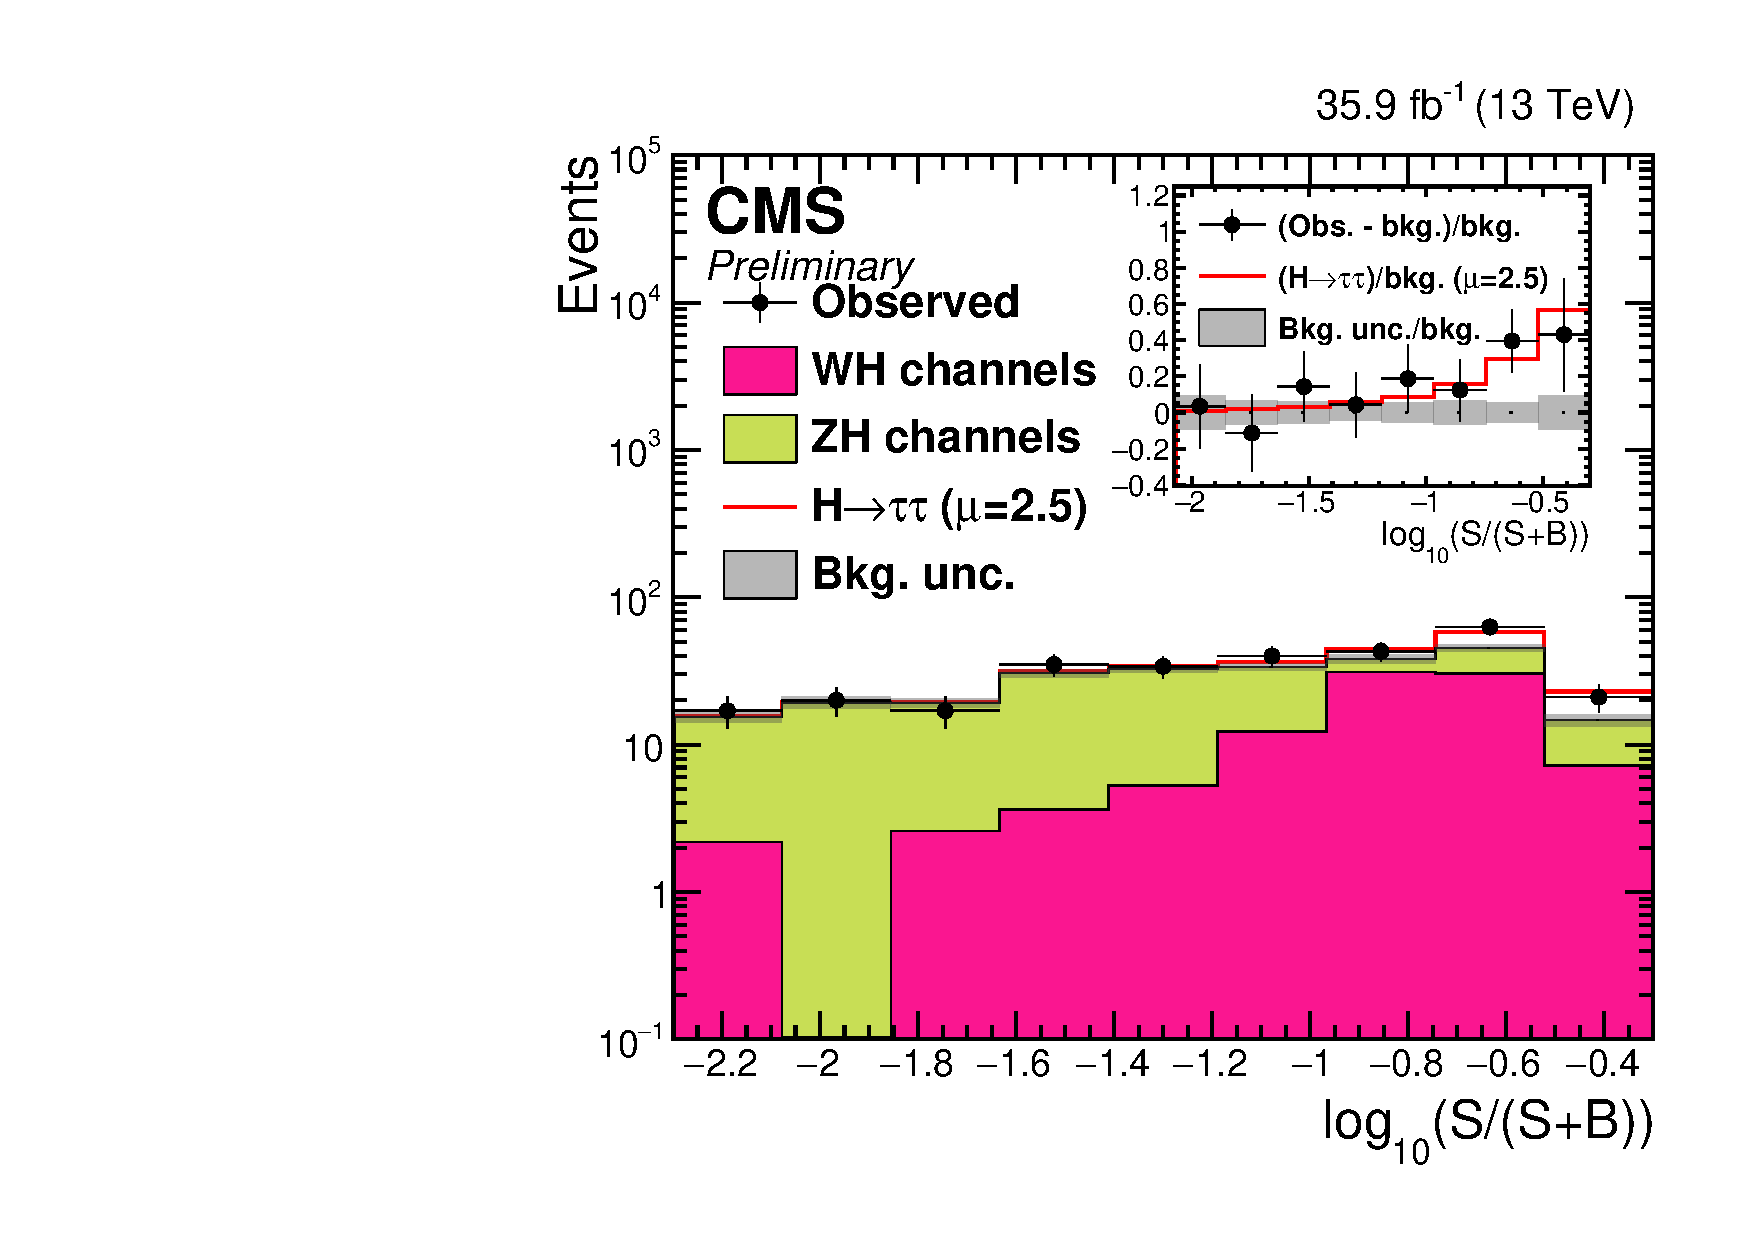
\includegraphics[width=0.45\textwidth]{higgs_to_taus_vh/plots/combined/wh_vs_zh_sbweight.pdf}
 \end{center}
 \caption{
 Distribution of the decimal logarithm of the ratio between the expected signal and the 
 sum of expected signal and expected background in each bin of the mass distributions 
 used to extract the results, in all signal regions. The background contributions are 
 separated based on the final state channels, $\PW\PH$ versus $\PZ\PH$. The inset 
 shows the corresponding difference between the 
 observed data and expected background distributions divided by the background expectation, 
 as well as the signal expectation divided by the background expectation.
 }
 \label{fig:sb}
\end{figure}



The best fit signal
strength from this dedicated $\PW\PH$ and $\PZ\PH$ associated production analysis is 
$\mu = 2.54 ^{+1.35} _{-1.26}$ ($\mu = 1.00 ^{+1.08} _{-0.97}$ expected) 
for a significance of 2.3 standard deviations (1.0 expected).

To fully exploit the $\PH \to \Pgt\Pgt$ data in the 2016 CMS dataset, the results
of this dedicated $\PW\PH$ and $\PZ\PH$ associated production analysis are combined with the prior
$\PH \to \Pgt\Pgt$ analysis~\cite{HIG-16-043}, which targeted the Gluon Fusion and
VBF Higgs boson production processes. 
%The combined results of these two analyses
%is discussed in the following chapter, Combine $\htt$ Results~\ref{sec:results_cmb}.
By combining these two $\htt$ analyses of
2016 CMS data, we have signal regions targeted each of the four leading Higgs 
boson production processes. The resulting signal strenghts, significance and, Higgs
boson couplings can be probed with greater precision than either analysis alone.
The best fit signal strength for from the combination is $\mu = 1.24 ^{+0.29} _{-0.27}$.
For reference, the best fit signal strength for the $ggH$ and VBF targeted analysis
is $\mu = 1.09 ^{+0.27} _{-0.26}$.
The signal strength from the combination can be decomposed by Higgs boson production 
process, Fig.~\ref{fig:mu_higgs_processes}. The combination leads to an 
observed significance of 5.5 standard deviations (4.8 expected). 

\begin{figure}[!ht]
 \begin{center}
  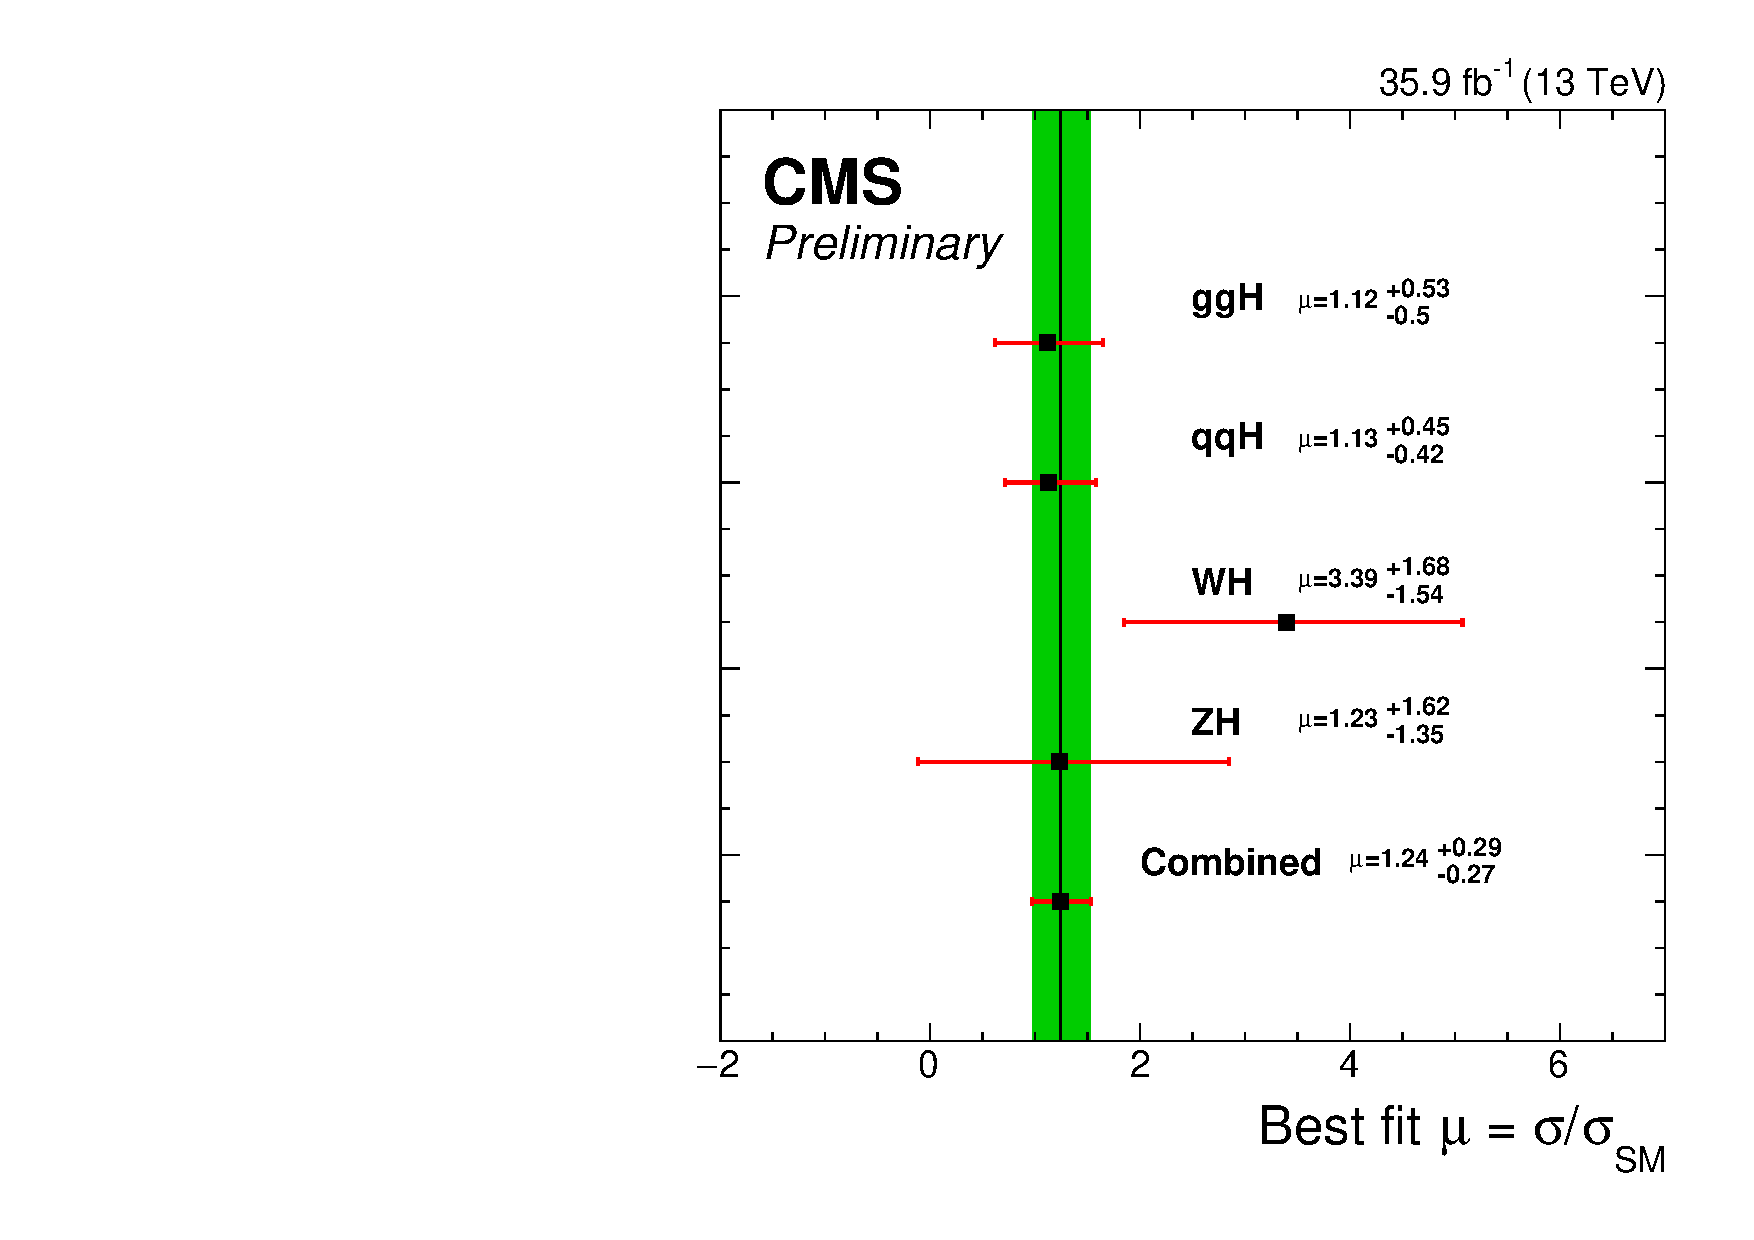
\includegraphics[width=0.45\textwidth]{higgs_to_taus_vh/plots/combined/mu_higgs_procs.pdf}
 \end{center}
 \caption{
 Best fit signal strength per $\PH$ production process, for $\mH = 125.09$\GeV.
 A combination of the $\PW\PH$ and $\PZ\PH$ analysis detailed in this paper
 with the $\htt$ CMS analysis~\cite{HIG-16-043} is used to
 fully exploit the $\htt$ data at CMS and constrain the
 Gluon Fusion and Vector Boson Scattering $\PH$ production processes as fully
 The constraints from the combined global fit are used to extract each of the 
 individual best fit signal strengths. The combined best fit signal strength 
 is $\mu = 1.24 ^{+0.29} _{-0.27}$.
 as is possible.
 }
 \label{fig:mu_higgs_processes}
\end{figure}

This same combination of this dedicated $\PW\PH$ and $\PZ\PH$ analysis with the prior
$\PH \to \Pgt\Pgt$ analysis~\cite{HIG-16-043}, can place the tightest
$\PH \to \Pgt\Pgt$ in the $(\kappa_\text{V}$,$\kappa_\text{f})$ parameter space.
A likelihood scan is performed for $\mH=125.09\GeV$ in the ($\kappa_\text{V}$,$\kappa_\text{f}$) 
parameter space, where $\kappa_\text{V}$ and $\kappa_\text{f}$ quantify, respectively, 
the ratio between the measured and the SM value for the couplings of the Higgs boson to 
vector bosons and fermions, with the methods described in Ref.~\cite{Chatrchyan:2014nva}. 
For this scan only, Higgs boson decays to pairs of $\PW$ or $\PZ$ bosons, $\hww$ or $\hzz$,
 are considered as part of 
the signal. The $\ttbar\PH$ production process is still treated as background because
the MC sample we use is not split by Higgs boson decay mode. All nuisance 
parameters are profiled for each point of the scan. As shown in 
Fig.~\ref{fig:kVkf}, the observed likelihood contour is consistent with the SM expectation 
of $\kappa_\text{V}$ and $\kappa_\text{f}$ equal to unity.

\begin{figure}[!ht]
 \begin{center}
  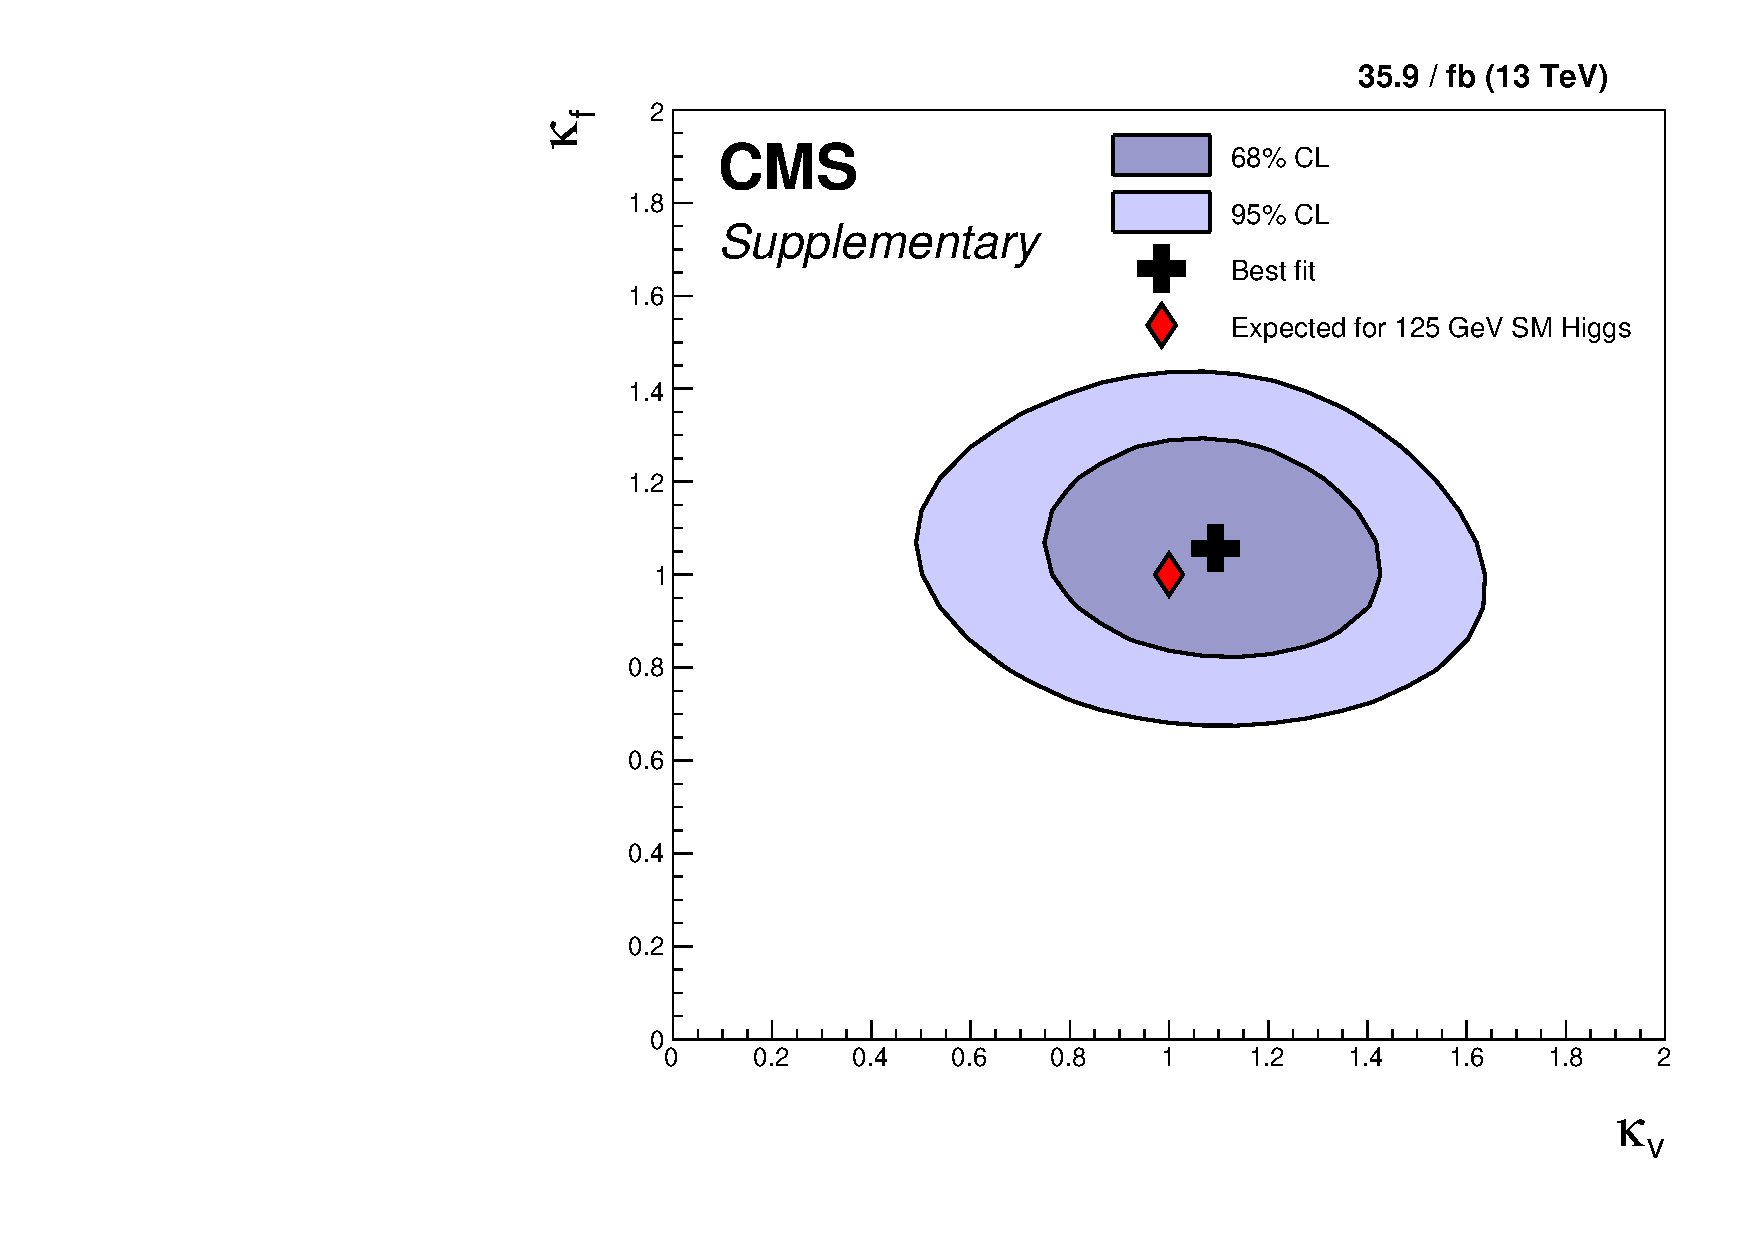
\includegraphics[width=0.45\textwidth]{higgs_to_taus_vh/plots/combined/kFkV_HIG-18-007_plus_HIG-16-043.pdf}
 \end{center}
 \caption{Scan of the negative 
 log-likelihood difference as a function of $\kappa_V$ and $\kappa_f$, for 
 $\mH = 125.09$\GeV.  All nuisance parameters are profiled for each point. 
 This scan is a combination of the $\PW\PH$ and $\PZ\PH$ targeted analysis detailed in this paper
 with the $\htt$ CMS analysis~\cite{HIG-16-043}.
 For this scan, the included $\hww$ and $\hzz$ production processes 
 are treated as signal processes.
 }
 \label{fig:kVkf}
\end{figure}



\section{Summary}
A search for the standard model Higgs boson based on data collected in proton-proton collisions by the
CMS detector in 2016 at a center-of-mass energy of 13\TeV focusing on the
two $\PW\PH$ and $\PZ\PH$ associated production processes has been presented. Event
categories have been split into three lepton final states targeting $\PW\PH$ production
and four lepton final states targeting $\PZ\PH$ production. The results are extracted
via maximum likelihood fits using the visible di-$\Pgt$ mass for the $\PW\PH$
channels and full di-$\Pgt$ mass for the $\PZ\PH$ channels. 
%Observed limits of 4.7 
%(expected 2.0) are placed on the Higgs boson associated production processes 
%times the SM prediction for a Higgs boson mass of 125.09\GeV. 
The best fit signal
strength is $\mu = 2.54 ^{+1.35} _{-1.26}$ ($\mu = 1.00 ^{+1.08} _{-0.97}$ expected) 
for a significance of 2.3 standard deviations (1.0 expected).

Combining this analysis with the previous 13\TeV $ggH$ and VFB targeted $\htt$ 
analysis~\cite{HIG-16-043}, we place the tightest constraints
on the $\htt$ process. 
The best fit signal strength is $\mu = 1.24 ^{+0.29} _{-0.27}$ leading to an
observed significance of 5.5 standard deviations (4.8 expected). 
The combination leads to a significant increase in constraint for the coupling
of the Higgs boson to vector bosons, the coupling to fermions is not greatly
affected. The resulting measured couplings are consistent with SM predictions
within one standard deviation.

\clearpage


